% Options for packages loaded elsewhere
\PassOptionsToPackage{unicode}{hyperref}
\PassOptionsToPackage{hyphens}{url}
%
\documentclass[
  ignorenonframetext,
]{beamer}
\usepackage{pgfpages}
\setbeamertemplate{caption}[numbered]
\setbeamertemplate{caption label separator}{: }
\setbeamercolor{caption name}{fg=normal text.fg}
\beamertemplatenavigationsymbolsempty
% Prevent slide breaks in the middle of a paragraph
\widowpenalties 1 10000
\raggedbottom
\setbeamertemplate{part page}{
  \centering
  \begin{beamercolorbox}[sep=16pt,center]{part title}
    \usebeamerfont{part title}\insertpart\par
  \end{beamercolorbox}
}
\setbeamertemplate{section page}{
  \centering
  \begin{beamercolorbox}[sep=12pt,center]{part title}
    \usebeamerfont{section title}\insertsection\par
  \end{beamercolorbox}
}
\setbeamertemplate{subsection page}{
  \centering
  \begin{beamercolorbox}[sep=8pt,center]{part title}
    \usebeamerfont{subsection title}\insertsubsection\par
  \end{beamercolorbox}
}
\AtBeginPart{
  \frame{\partpage}
}
\AtBeginSection{
  \ifbibliography
  \else
    \frame{\sectionpage}
  \fi
}
\AtBeginSubsection{
  \frame{\subsectionpage}
}

\usepackage{amsmath,amssymb}
\usepackage{iftex}
\ifPDFTeX
  \usepackage[T1]{fontenc}
  \usepackage[utf8]{inputenc}
  \usepackage{textcomp} % provide euro and other symbols
\else % if luatex or xetex
  \usepackage{unicode-math}
  \defaultfontfeatures{Scale=MatchLowercase}
  \defaultfontfeatures[\rmfamily]{Ligatures=TeX,Scale=1}
\fi
\usepackage{lmodern}
\ifPDFTeX\else  
    % xetex/luatex font selection
\fi
% Use upquote if available, for straight quotes in verbatim environments
\IfFileExists{upquote.sty}{\usepackage{upquote}}{}
\IfFileExists{microtype.sty}{% use microtype if available
  \usepackage[]{microtype}
  \UseMicrotypeSet[protrusion]{basicmath} % disable protrusion for tt fonts
}{}
\makeatletter
\@ifundefined{KOMAClassName}{% if non-KOMA class
  \IfFileExists{parskip.sty}{%
    \usepackage{parskip}
  }{% else
    \setlength{\parindent}{0pt}
    \setlength{\parskip}{6pt plus 2pt minus 1pt}}
}{% if KOMA class
  \KOMAoptions{parskip=half}}
\makeatother
\usepackage{xcolor}
\newif\ifbibliography
\setlength{\emergencystretch}{3em} % prevent overfull lines
\setcounter{secnumdepth}{-\maxdimen} % remove section numbering


\providecommand{\tightlist}{%
  \setlength{\itemsep}{0pt}\setlength{\parskip}{0pt}}\usepackage{longtable,booktabs,array}
\usepackage{calc} % for calculating minipage widths
\usepackage{caption}
% Make caption package work with longtable
\makeatletter
\def\fnum@table{\tablename~\thetable}
\makeatother
\usepackage{graphicx}
\makeatletter
\def\maxwidth{\ifdim\Gin@nat@width>\linewidth\linewidth\else\Gin@nat@width\fi}
\def\maxheight{\ifdim\Gin@nat@height>\textheight\textheight\else\Gin@nat@height\fi}
\makeatother
% Scale images if necessary, so that they will not overflow the page
% margins by default, and it is still possible to overwrite the defaults
% using explicit options in \includegraphics[width, height, ...]{}
\setkeys{Gin}{width=\maxwidth,height=\maxheight,keepaspectratio}
% Set default figure placement to htbp
\makeatletter
\def\fps@figure{htbp}
\makeatother

\usepackage{booktabs}
\usepackage{longtable}
\usepackage{array}
\usepackage{multirow}
\usepackage{wrapfig}
\usepackage{float}
\usepackage{colortbl}
\usepackage{pdflscape}
\usepackage{tabu}
\usepackage{threeparttable}
\usepackage{threeparttablex}
\usepackage[normalem]{ulem}
\usepackage{makecell}
\usepackage{xcolor}
\usepackage{tabularray}
\usepackage[normalem]{ulem}
\usepackage{graphicx}
\UseTblrLibrary{booktabs}
\UseTblrLibrary{siunitx}
\NewTableCommand{\tinytableDefineColor}[3]{\definecolor{#1}{#2}{#3}}
\newcommand{\tinytableTabularrayUnderline}[1]{\underline{#1}}
\newcommand{\tinytableTabularrayStrikeout}[1]{\sout{#1}}
\makeatletter
\@ifpackageloaded{caption}{}{\usepackage{caption}}
\AtBeginDocument{%
\ifdefined\contentsname
  \renewcommand*\contentsname{Table of contents}
\else
  \newcommand\contentsname{Table of contents}
\fi
\ifdefined\listfigurename
  \renewcommand*\listfigurename{List of Figures}
\else
  \newcommand\listfigurename{List of Figures}
\fi
\ifdefined\listtablename
  \renewcommand*\listtablename{List of Tables}
\else
  \newcommand\listtablename{List of Tables}
\fi
\ifdefined\figurename
  \renewcommand*\figurename{Figure}
\else
  \newcommand\figurename{Figure}
\fi
\ifdefined\tablename
  \renewcommand*\tablename{Table}
\else
  \newcommand\tablename{Table}
\fi
}
\@ifpackageloaded{float}{}{\usepackage{float}}
\floatstyle{ruled}
\@ifundefined{c@chapter}{\newfloat{codelisting}{h}{lop}}{\newfloat{codelisting}{h}{lop}[chapter]}
\floatname{codelisting}{Listing}
\newcommand*\listoflistings{\listof{codelisting}{List of Listings}}
\makeatother
\makeatletter
\makeatother
\makeatletter
\@ifpackageloaded{caption}{}{\usepackage{caption}}
\@ifpackageloaded{subcaption}{}{\usepackage{subcaption}}
\makeatother

\ifLuaTeX
  \usepackage{selnolig}  % disable illegal ligatures
\fi
\usepackage{bookmark}

\IfFileExists{xurl.sty}{\usepackage{xurl}}{} % add URL line breaks if available
\urlstyle{same} % disable monospaced font for URLs
\hypersetup{
  pdftitle={Gráficos},
  pdfauthor={Victor Batista},
  hidelinks,
  pdfcreator={LaTeX via pandoc}}


\title{Gráficos}
\author{Victor Batista}
\date{}

\begin{document}
\frame{\titlepage}


\begin{frame}{Mapa por grupos}
\phantomsection\label{mapa-por-grupos}
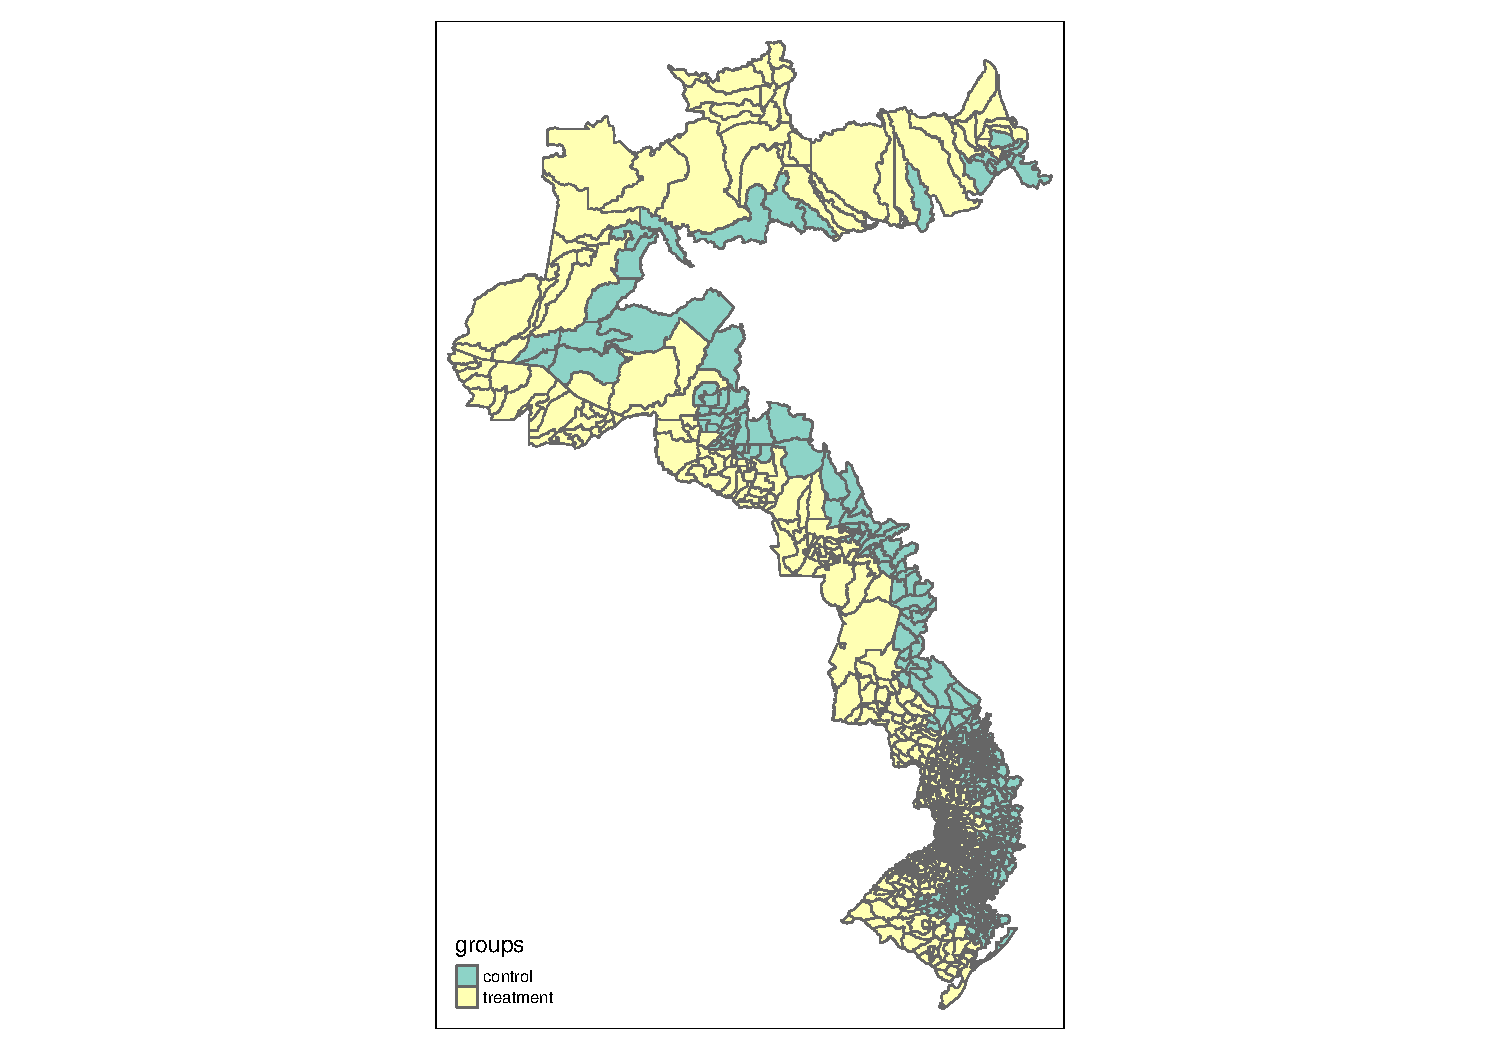
\includegraphics{graficos_files/figure-beamer/unnamed-chunk-4-1.pdf}
\end{frame}

\begin{frame}{Mapa por arcos}
\phantomsection\label{mapa-por-arcos}
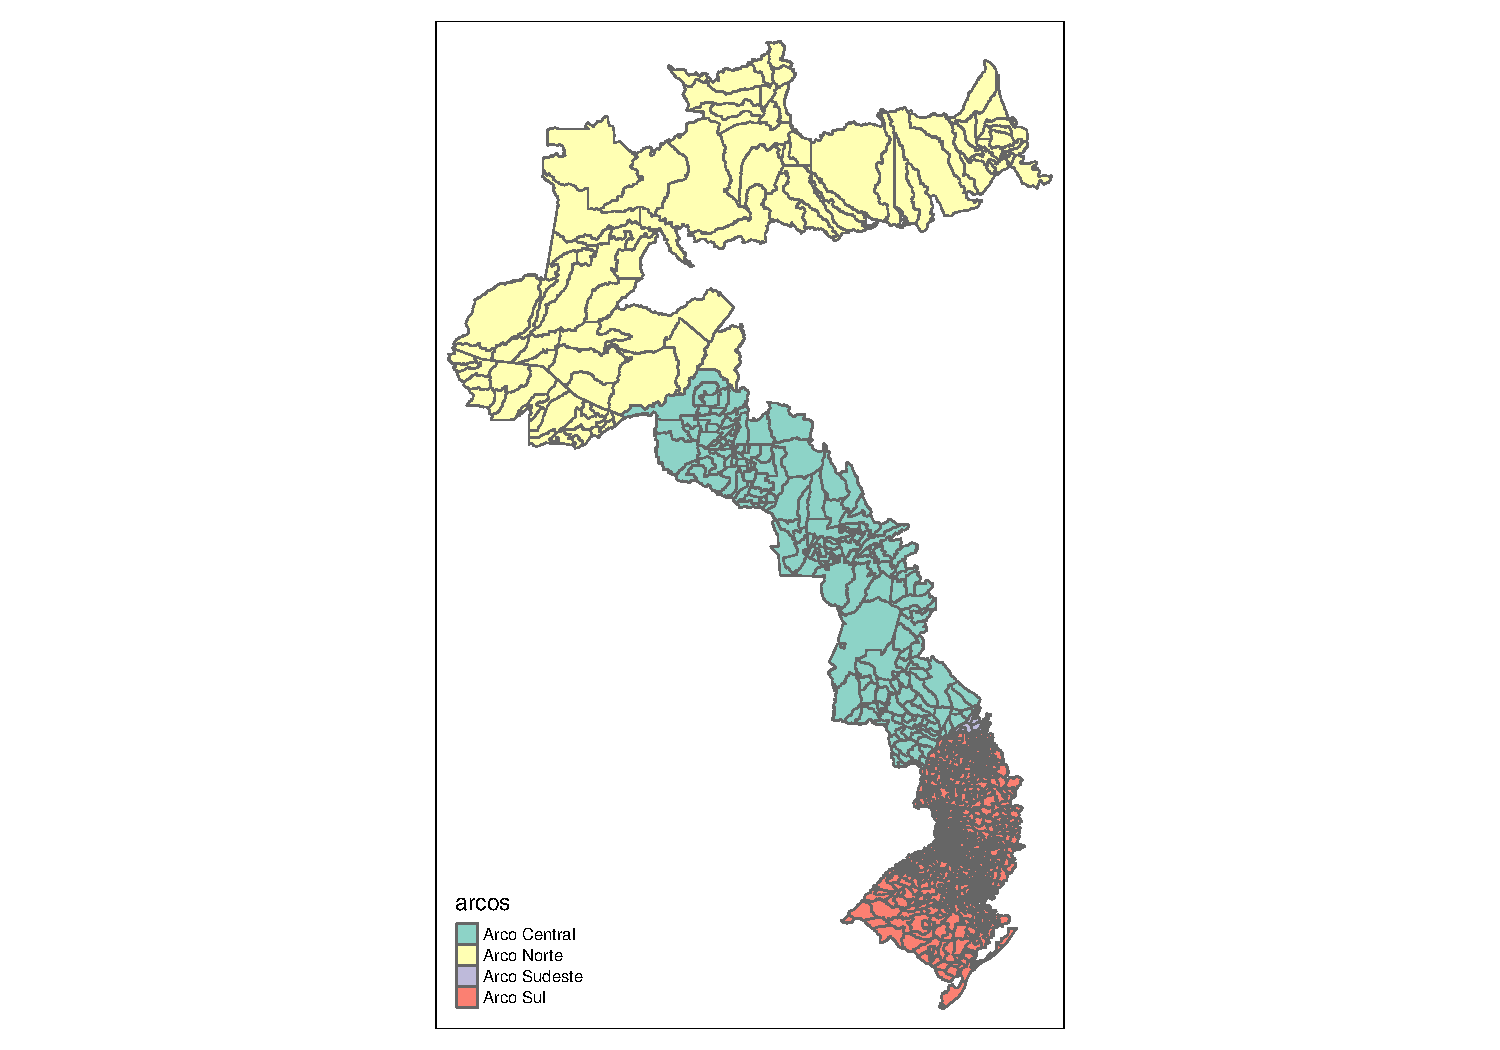
\includegraphics{graficos_files/figure-beamer/unnamed-chunk-5-1.pdf}
\end{frame}

\section{Análise exploratória}\label{anuxe1lise-exploratuxf3ria}

\begin{frame}{Estatísticas descritivas}
\phantomsection\label{estatuxedsticas-descritivas}
\begin{table}
\centering
\begin{tblr}[         %% tabularray outer open
]                     %% tabularray outer close
{                     %% tabularray inner open
colspec={Q[]Q[]Q[]Q[]Q[]Q[]Q[]Q[]Q[]},
hline{28}={1,2,3,4,5,6,7,8,9}{solid, 0.1em, black},
}                     %% tabularray inner close
\toprule
& Unique & Missing Pct. & Mean & SD & Min & Median & Max & Histogram \\ \midrule %% TinyTableHeader
Taxa\_de\_analfabetismo & 220 & 0 & 9.9 & 5.7 & 0.9 & 9.1 & 40.2 & 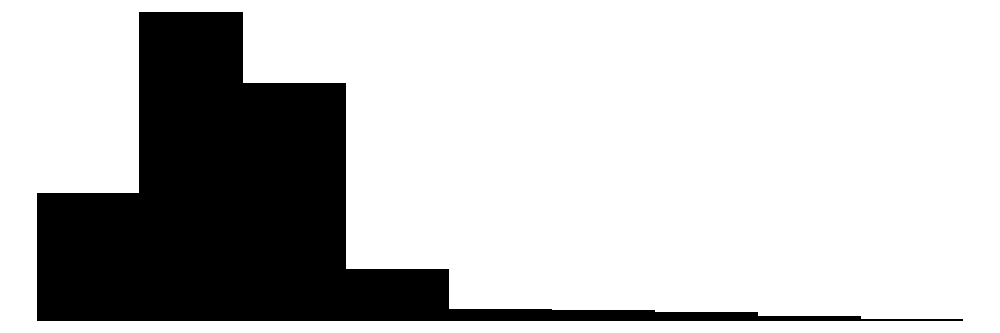
\includegraphics[height=1em]{tinytable_assets/idje2o3tmmvstuhqmr5jhg.png} \\
Taxa\_de\_desemprego\_16a\_e+ & 643 & 0 & 4.1 & 2.7 & 0.1 & 3.8 & 27.8 & 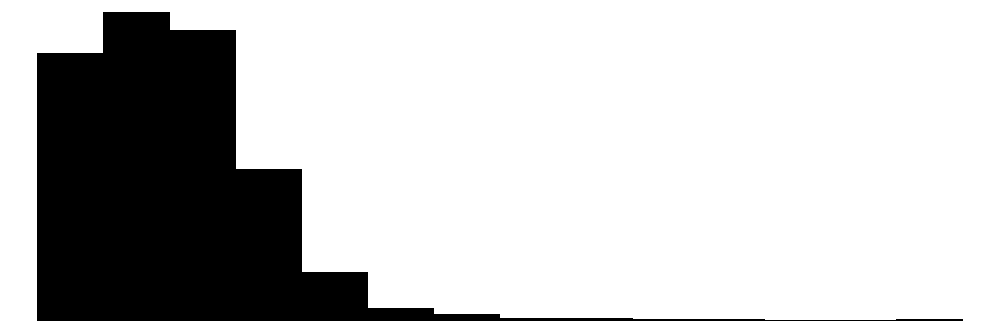
\includegraphics[height=1em]{tinytable_assets/idm6aeknzse0ebt03tbt35.png} \\
Gini & 898 & 0 & 0.5 & 0.1 & 0.3 & 0.5 & 0.8 & 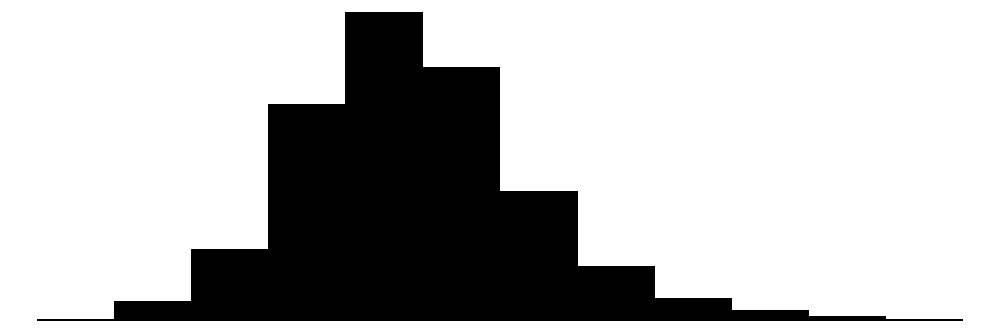
\includegraphics[height=1em]{tinytable_assets/idwqc7j4u7n21tbe2j3fpz.png} \\
PIB\_per\_capita & 1130 & 0 & 16374.5 & 12533.7 & 3129.3 & 13963.5 & 220358.3 & 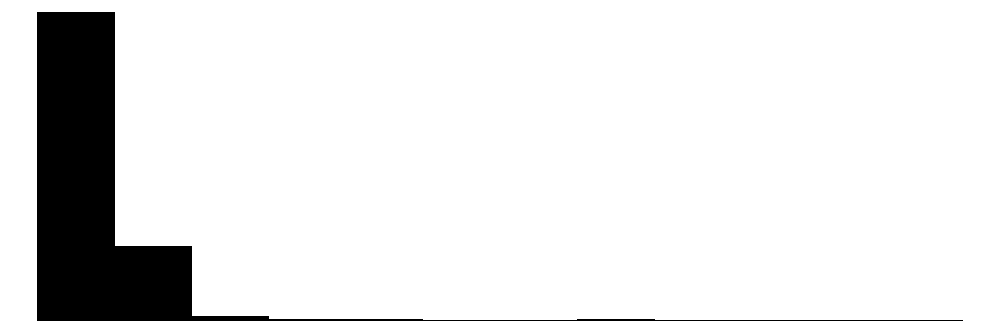
\includegraphics[height=1em]{tinytable_assets/idy08xykl0nlysmgwcao4g.png} \\
\%\_população\_com\_renda\_<\_1/4\_SM & 934 & 0 & 13.9 & 13.0 & 0.1 & 9.9 & 77.9 & 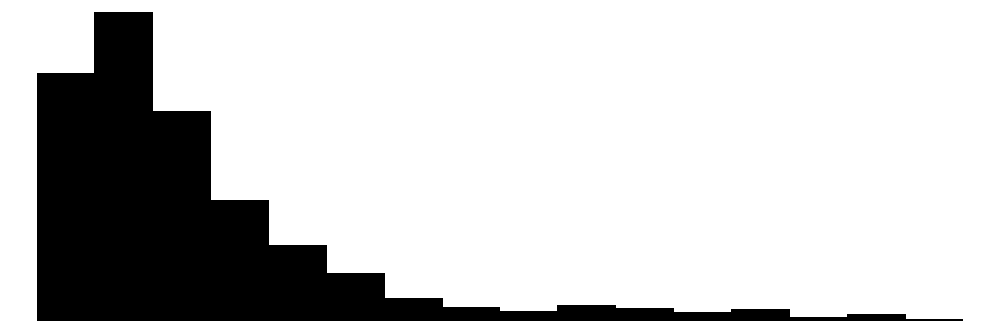
\includegraphics[height=1em]{tinytable_assets/idgb7p6esgqlj3bqnhup0u.png} \\
Taxa\_de\_trabalho\_infantil & 932 & 0 & 17.2 & 10.8 & 0.3 & 14.5 & 72.1 & 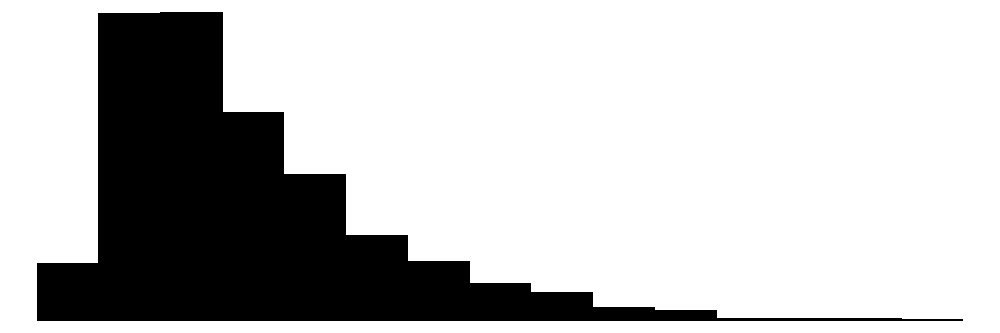
\includegraphics[height=1em]{tinytable_assets/id2hi3wff6yjqta15b6s06.png} \\
Porcentagem\_Homens\_Jovens & 498 & 0 & 12.5 & 1.5 & 7.9 & 12.4 & 26.7 & 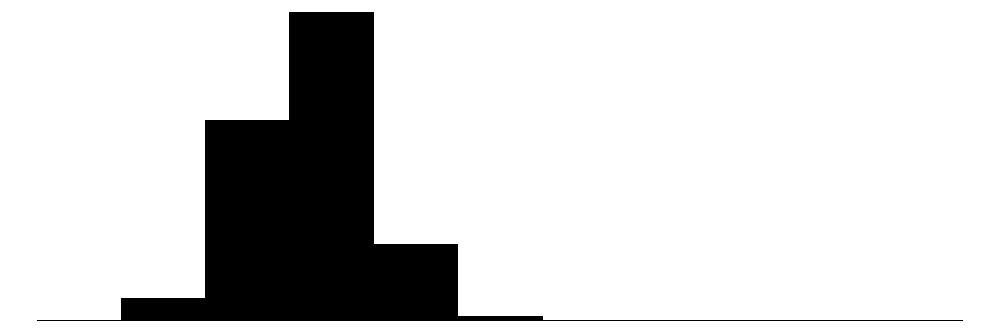
\includegraphics[height=1em]{tinytable_assets/id0gul6266fhzf3zjd08jq.png} \\
valor-2010 & 658 & 0 & 15.5 & 18.7 & 0.0 & 10.2 & 147.4 & 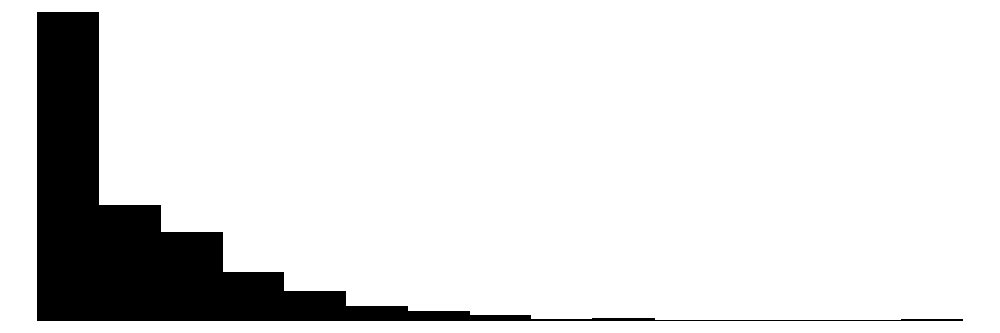
\includegraphics[height=1em]{tinytable_assets/id74js6ppc2qnnheex4z6s.png} \\
valor-2011 & 620 & 0 & 14.1 & 17.3 & 0.0 & 9.1 & 111.1 & 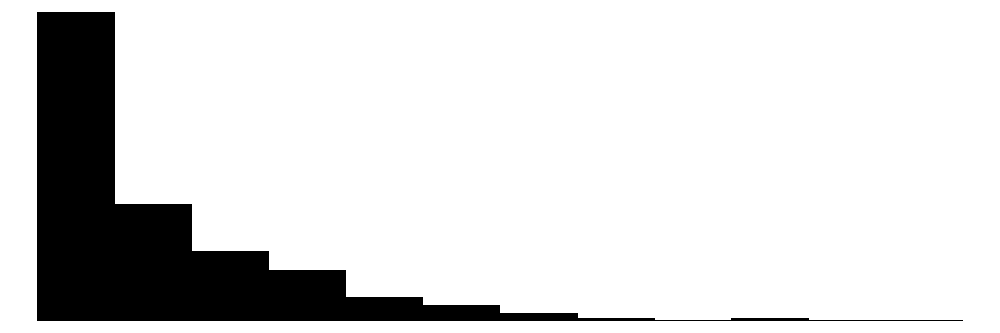
\includegraphics[height=1em]{tinytable_assets/id24cx3ig2v5n9h88ty5l0.png} \\
valor-2012 & 648 & 0 & 16.1 & 19.3 & 0.0 & 10.9 & 132.0 & 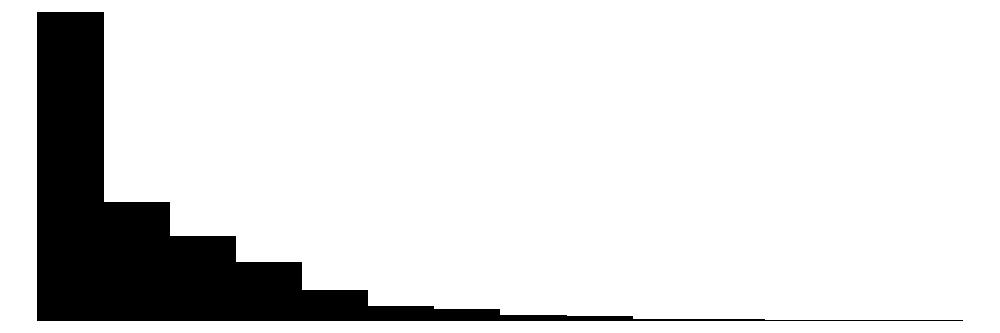
\includegraphics[height=1em]{tinytable_assets/idfk8jbweic3tb4ssdpbcq.png} \\
valor-2013 & 662 & 0 & 15.9 & 19.8 & 0.0 & 11.7 & 183.7 & 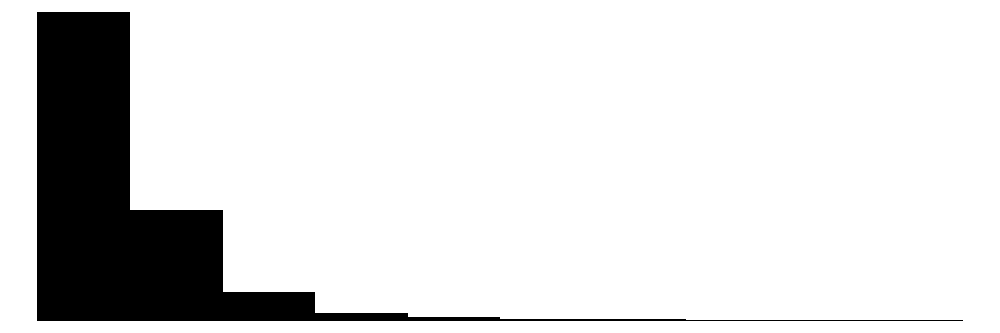
\includegraphics[height=1em]{tinytable_assets/idu7ab9hlfvf1v64xjr5oc.png} \\
valor-2014 & 680 & 0 & 16.4 & 19.0 & 0.0 & 11.8 & 153.9 & 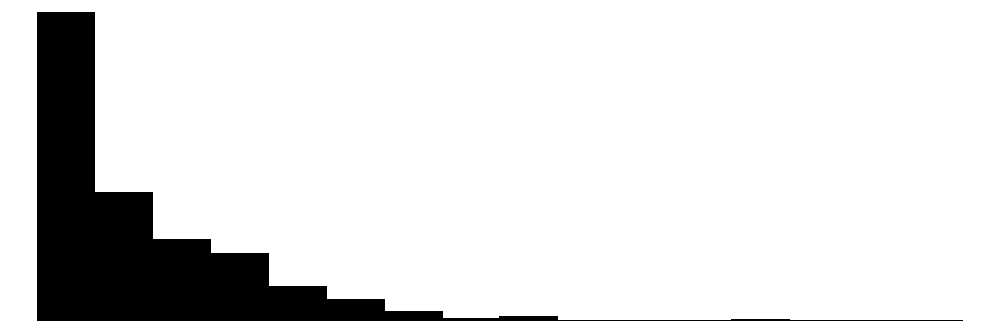
\includegraphics[height=1em]{tinytable_assets/iddn0vjvggqi9f71rgalmw.png} \\
valor-2015 & 671 & 0 & 16.5 & 19.1 & 0.0 & 11.8 & 137.1 & 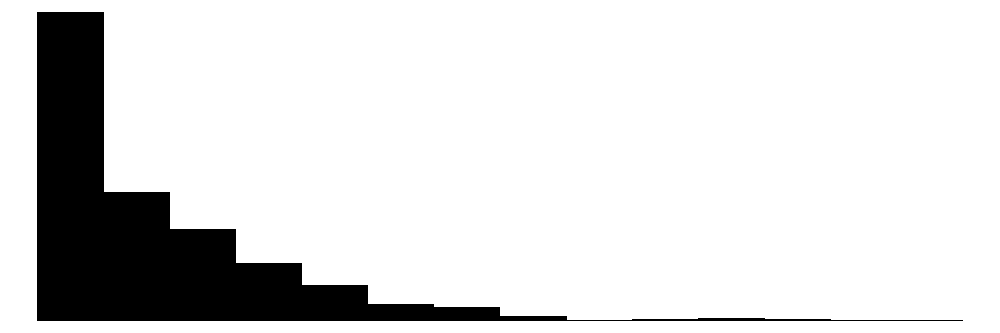
\includegraphics[height=1em]{tinytable_assets/idsn4yiarnynxrvvzc7cc6.png} \\
valor-2016 & 690 & 0 & 18.2 & 20.7 & 0.0 & 13.2 & 155.1 & 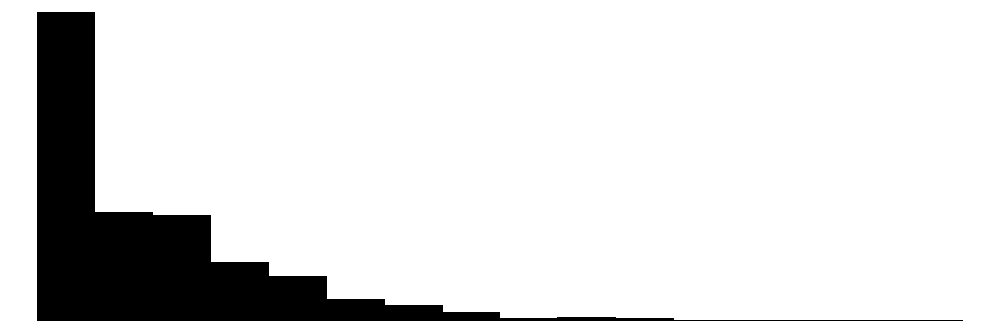
\includegraphics[height=1em]{tinytable_assets/idkclr7hrlvfwan7446pu7.png} \\
valor-2017 & 706 & 0 & 19.6 & 22.2 & 0.0 & 14.6 & 222.0 & 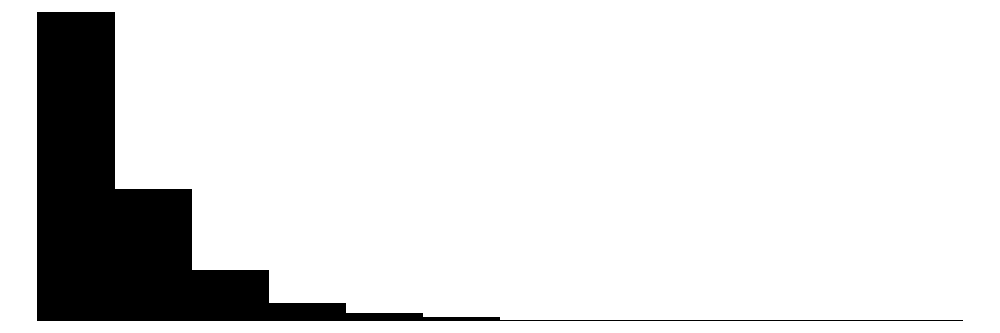
\includegraphics[height=1em]{tinytable_assets/idabmpedosye0slv9si8ka.png} \\
valor-2018 & 678 & 0 & 16.9 & 20.3 & 0.0 & 12.4 & 211.0 & 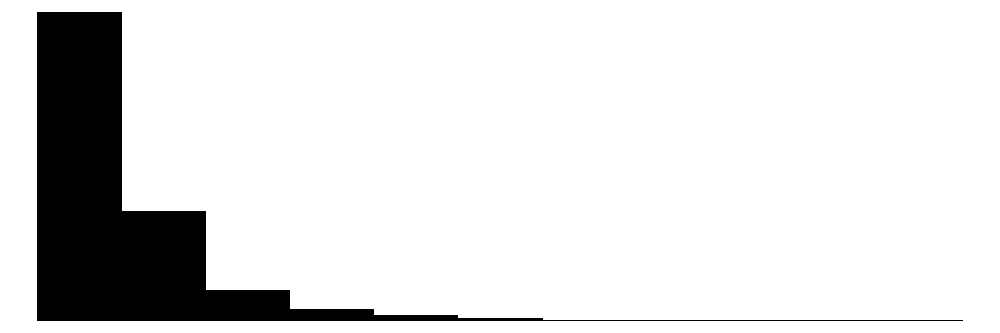
\includegraphics[height=1em]{tinytable_assets/idfh7pbnxsd6bsz5ztx52r.png} \\
valor-2019 & 657 & 0 & 15.5 & 19.2 & 0.0 & 10.9 & 176.7 & 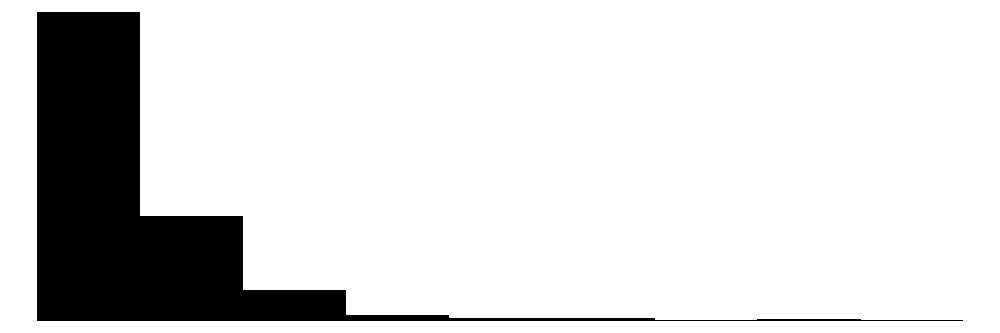
\includegraphics[height=1em]{tinytable_assets/id5zd3pcthhz940t1by4w6.png} \\
populacao & 1100 & 0 & 22568.3 & 70848.0 & 1034.0 & 7593.0 & 1483771.0 & 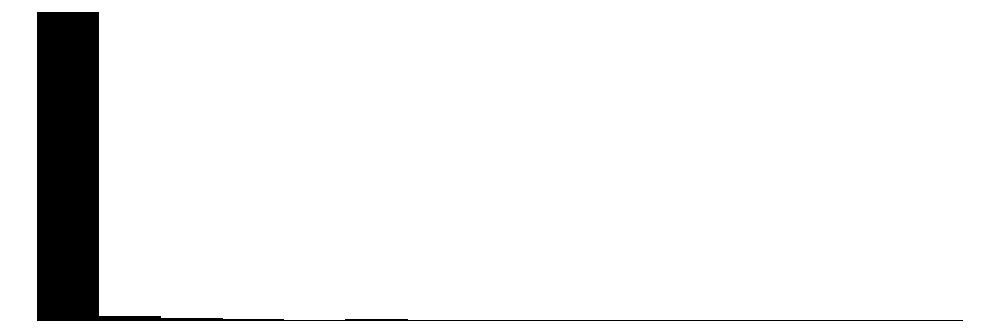
\includegraphics[height=1em]{tinytable_assets/id7rf4k25zla3esfpsd88y.png} \\
feminicidio\_pc & 156 & 0 & 1.4 & 6.5 & 0.0 & 0.0 & 101.7 & 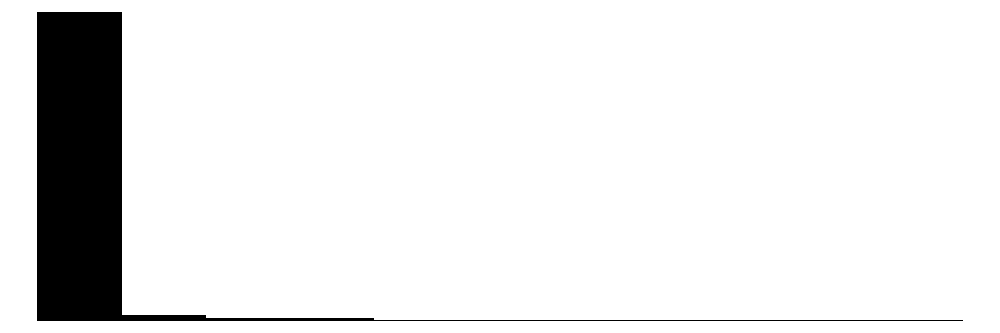
\includegraphics[height=1em]{tinytable_assets/idaragmu4uks39uup9hy2b.png} \\
hom\_doloso\_pc & 621 & 0 & 31.7 & 263.5 & 0.0 & 6.0 & 8203.4 & 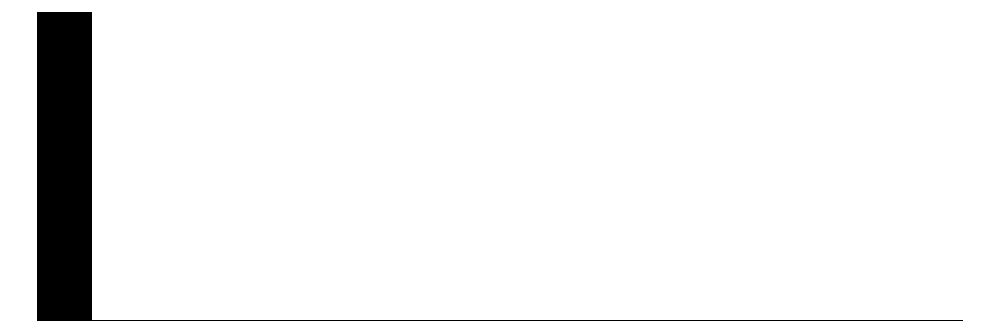
\includegraphics[height=1em]{tinytable_assets/idb2nnx3hnatb4s5iawmsi.png} \\
lesao\_pc & 74 & 0 & 0.9 & 6.9 & 0.0 & 0.0 & 169.5 & 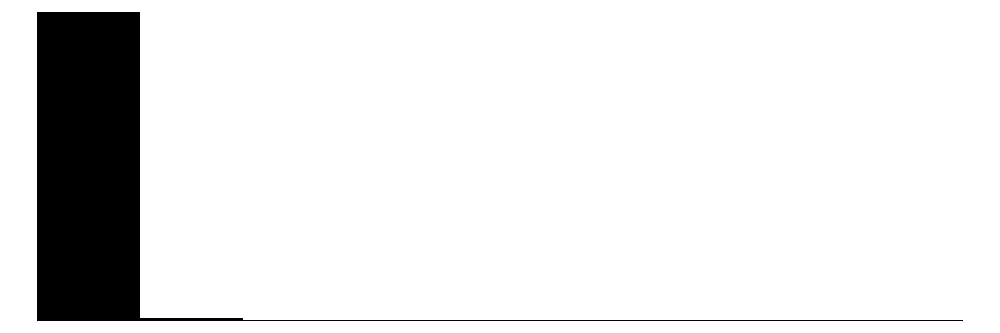
\includegraphics[height=1em]{tinytable_assets/idkb2kvudlm71o04dw4eu4.png} \\
mandado\_pc & 625 & 0 & 98.5 & 173.8 & 0.0 & 21.1 & 1285.4 & 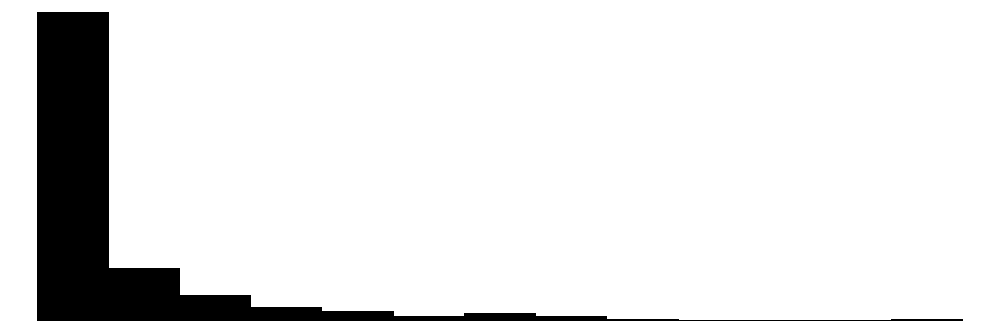
\includegraphics[height=1em]{tinytable_assets/idmuzn83i8e6bb2v9gmrn9.png} \\
transito\_pc & 588 & 0 & 20.1 & 86.6 & 0.0 & 3.2 & 2474.6 & 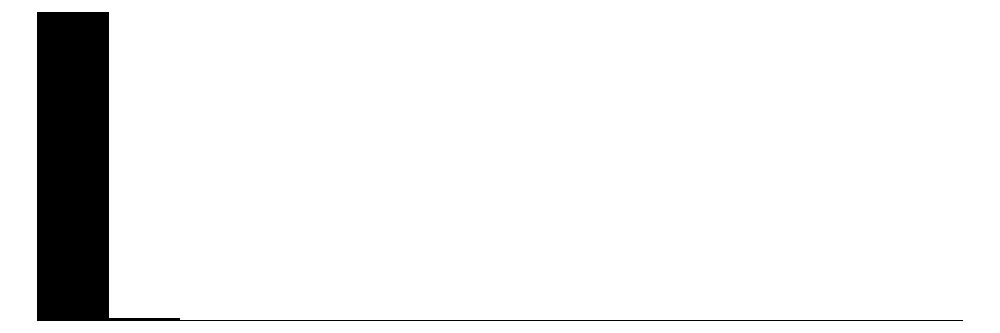
\includegraphics[height=1em]{tinytable_assets/idss5abzqvmblin5yhos5m.png} \\
esclarecer\_pc & 531 & 0 & 58.4 & 1096.0 & 0.0 & 0.0 & 36508.5 & 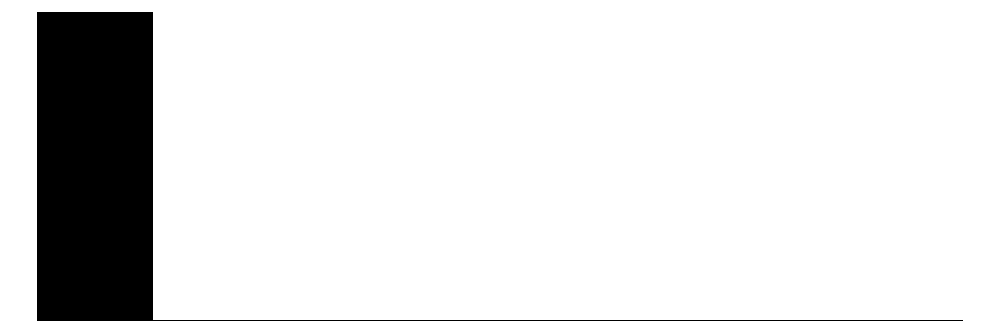
\includegraphics[height=1em]{tinytable_assets/idut0pmhrsic70kg7km70r.png} \\
latrocinio\_pc & 138 & 0 & 1.7 & 11.4 & 0.0 & 0.0 & 305.1 & 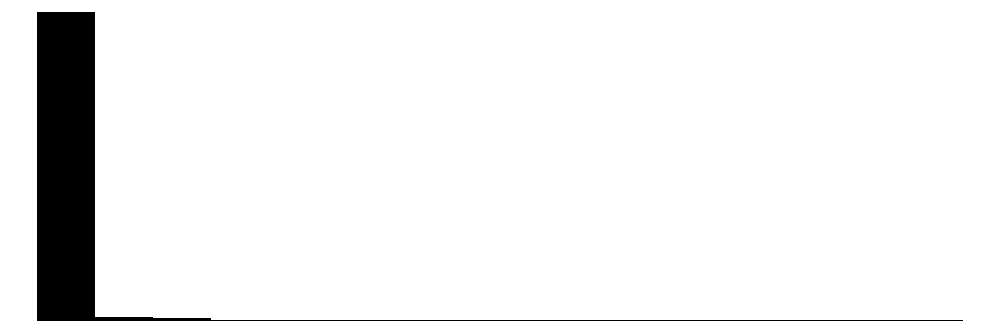
\includegraphics[height=1em]{tinytable_assets/idgfellqoxr8clyz01cfxc.png} \\
tentativa\_hom\_pc & 570 & 0 & 26.8 & 164.6 & 0.0 & 2.3 & 4678.0 & 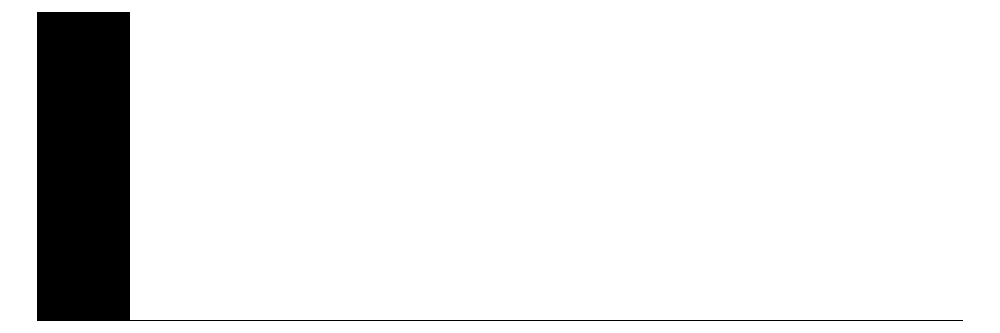
\includegraphics[height=1em]{tinytable_assets/idey62gjqw35hm6xhdmrga.png} \\
&    & N & \% &  &  &  &  &  \\
code\_state & 11 & 52 & 4.6 &  &  &  &  &  \\
& 12 & 22 & 1.9 &  &  &  &  &  \\
& 13 & 32 & 2.8 &  &  &  &  &  \\
& 14 & 15 & 1.3 &  &  &  &  &  \\
& 15 & 7 & 0.6 &  &  &  &  &  \\
& 16 & 15 & 1.3 &  &  &  &  &  \\
& 35 & 12 & 1.1 &  &  &  &  &  \\
& 41 & 297 & 26.2 &  &  &  &  &  \\
& 42 & 144 & 12.7 &  &  &  &  &  \\
& 43 & 413 & 36.5 &  &  &  &  &  \\
& 50 & 66 & 5.8 &  &  &  &  &  \\
& 51 & 57 & 5.0 &  &  &  &  &  \\
abbrev\_state & AC & 22 & 1.9 &  &  &  &  &  \\
& AM & 32 & 2.8 &  &  &  &  &  \\
& AP & 15 & 1.3 &  &  &  &  &  \\
& MS & 66 & 5.8 &  &  &  &  &  \\
& MT & 57 & 5.0 &  &  &  &  &  \\
& PA & 7 & 0.6 &  &  &  &  &  \\
& PR & 297 & 26.2 &  &  &  &  &  \\
& RO & 52 & 4.6 &  &  &  &  &  \\
& RR & 15 & 1.3 &  &  &  &  &  \\
& RS & 413 & 36.5 &  &  &  &  &  \\
& SC & 144 & 12.7 &  &  &  &  &  \\
& SP & 12 & 1.1 &  &  &  &  &  \\
name\_state & Acre & 22 & 1.9 &  &  &  &  &  \\
& Amapá & 15 & 1.3 &  &  &  &  &  \\
& Amazônas & 32 & 2.8 &  &  &  &  &  \\
& Mato Grosso & 57 & 5.0 &  &  &  &  &  \\
& Mato Grosso do Sul & 66 & 5.8 &  &  &  &  &  \\
& Pará & 7 & 0.6 &  &  &  &  &  \\
& Paraná & 297 & 26.2 &  &  &  &  &  \\
& Rio Grande do Sul & 413 & 36.5 &  &  &  &  &  \\
& Rondônia & 52 & 4.6 &  &  &  &  &  \\
& Roraima & 15 & 1.3 &  &  &  &  &  \\
& Santa Catarina & 144 & 12.7 &  &  &  &  &  \\
& São Paulo & 12 & 1.1 &  &  &  &  &  \\
code\_region & 1 & 143 & 12.6 &  &  &  &  &  \\
& 3 & 12 & 1.1 &  &  &  &  &  \\
& 4 & 854 & 75.4 &  &  &  &  &  \\
& 5 & 123 & 10.9 &  &  &  &  &  \\
name\_region & Centro Oeste & 123 & 10.9 &  &  &  &  &  \\
& Norte & 143 & 12.6 &  &  &  &  &  \\
& Sudeste & 12 & 1.1 &  &  &  &  &  \\
& Sul & 854 & 75.4 &  &  &  &  &  \\
fronteira & FALSE & 544 & 48.1 &  &  &  &  &  \\
& TRUE & 588 & 51.9 &  &  &  &  &  \\
treated & FALSE & 544 & 48.1 &  &  &  &  &  \\
& TRUE & 588 & 51.9 &  &  &  &  &  \\
groups & control & 544 & 48.1 &  &  &  &  &  \\
& treatment & 588 & 51.9 &  &  &  &  &  \\
arcos & Arco Central & 175 & 15.5 &  &  &  &  &  \\
& Arco Norte & 91 & 8.0 &  &  &  &  &  \\
& Arco Sul & 854 & 75.4 &  &  &  &  &  \\
& NA & 12 & 1.1 &  &  &  &  &  \\
CID\_GEMEA & FALSE & 555 & 49.0 &  &  &  &  &  \\
& TRUE & 33 & 2.9 &  &  &  &  &  \\
& NA & 544 & 48.1 &  &  &  &  &  \\
FAIXA\_SEDE & FALSE & 77 & 6.8 &  &  &  &  &  \\
& TRUE & 511 & 45.1 &  &  &  &  &  \\
& NA & 544 & 48.1 &  &  &  &  &  \\
Argentina & FALSE & 1099 & 97.1 &  &  &  &  &  \\
& TRUE & 33 & 2.9 &  &  &  &  &  \\
Bolivia & FALSE & 1112 & 98.2 &  &  &  &  &  \\
& TRUE & 20 & 1.8 &  &  &  &  &  \\
Colombia & FALSE & 1130 & 99.8 &  &  &  &  &  \\
& TRUE & 2 & 0.2 &  &  &  &  &  \\
French\_Guiana & FALSE & 1130 & 99.8 &  &  &  &  &  \\
& TRUE & 2 & 0.2 &  &  &  &  &  \\
Guyana & FALSE & 1126 & 99.5 &  &  &  &  &  \\
& TRUE & 6 & 0.5 &  &  &  &  &  \\
Suriname & FALSE & 1128 & 99.6 &  &  &  &  &  \\
& TRUE & 4 & 0.4 &  &  &  &  &  \\
Paraguay & FALSE & 1112 & 98.2 &  &  &  &  &  \\
& TRUE & 20 & 1.8 &  &  &  &  &  \\
Peru & FALSE & 1120 & 98.9 &  &  &  &  &  \\
& TRUE & 12 & 1.1 &  &  &  &  &  \\
Uruguay & FALSE & 1120 & 98.9 &  &  &  &  &  \\
& TRUE & 12 & 1.1 &  &  &  &  &  \\
Venezuela & FALSE & 1124 & 99.3 &  &  &  &  &  \\
& TRUE & 8 & 0.7 &  &  &  &  &  \\
\bottomrule
\end{tblr}
\end{table}
\end{frame}

\begin{frame}{Distribuição}
\phantomsection\label{distribuiuxe7uxe3o}
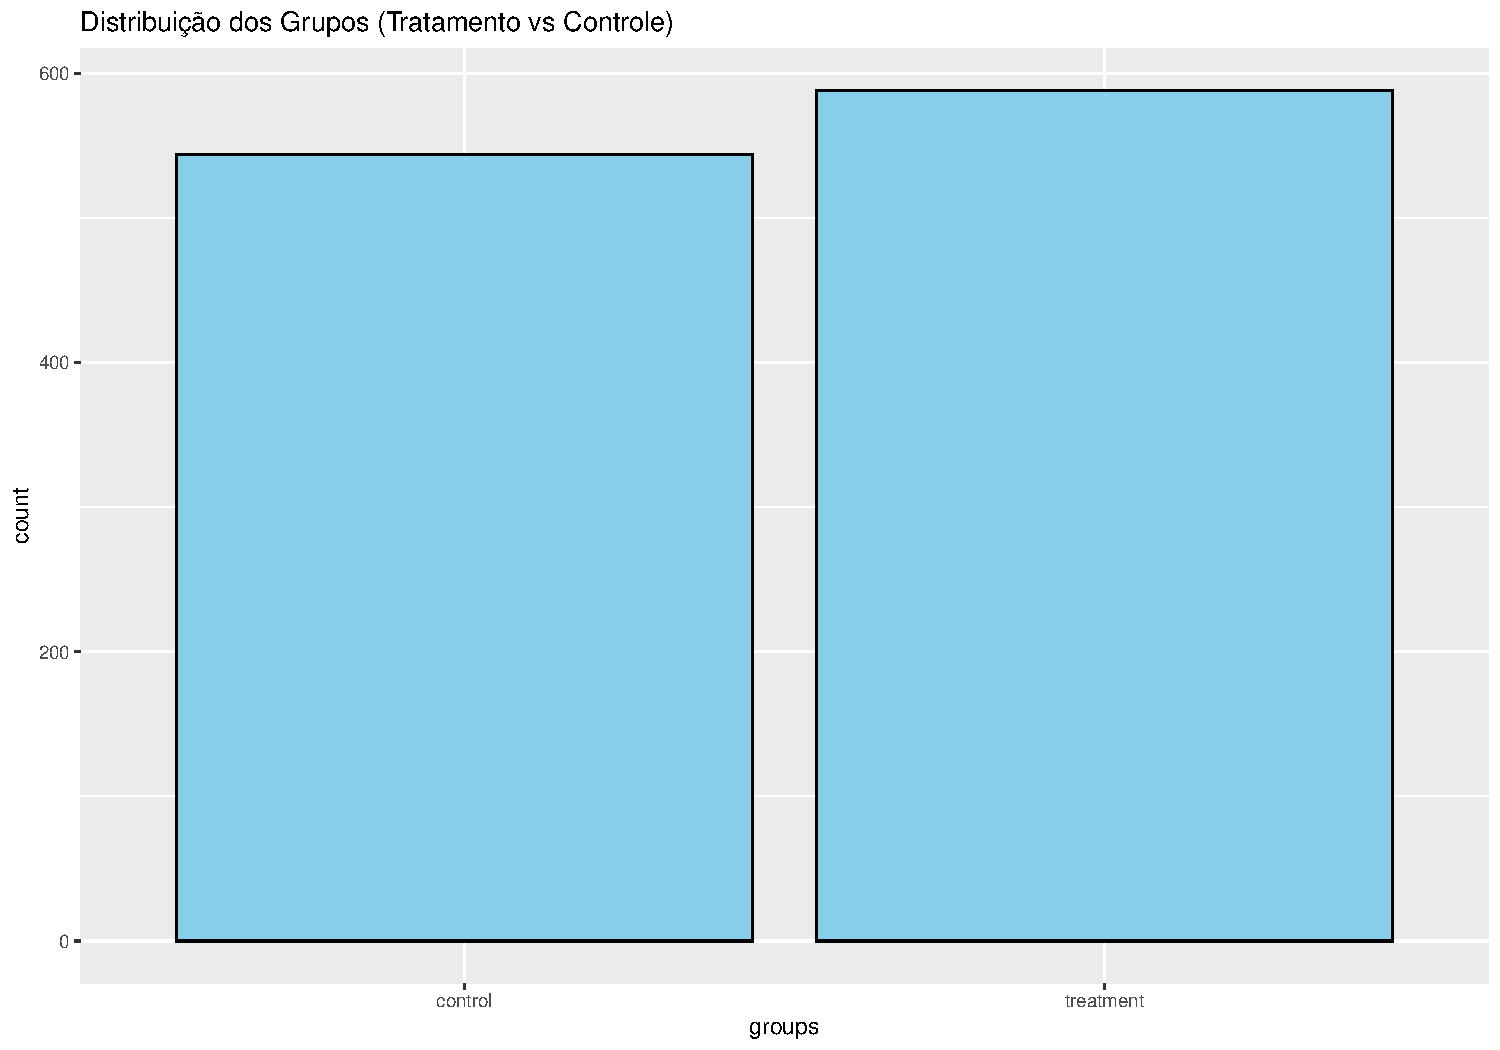
\includegraphics{graficos_files/figure-beamer/unnamed-chunk-8-1.pdf}
\end{frame}

\begin{frame}{Analfabetismo}
\phantomsection\label{analfabetismo}
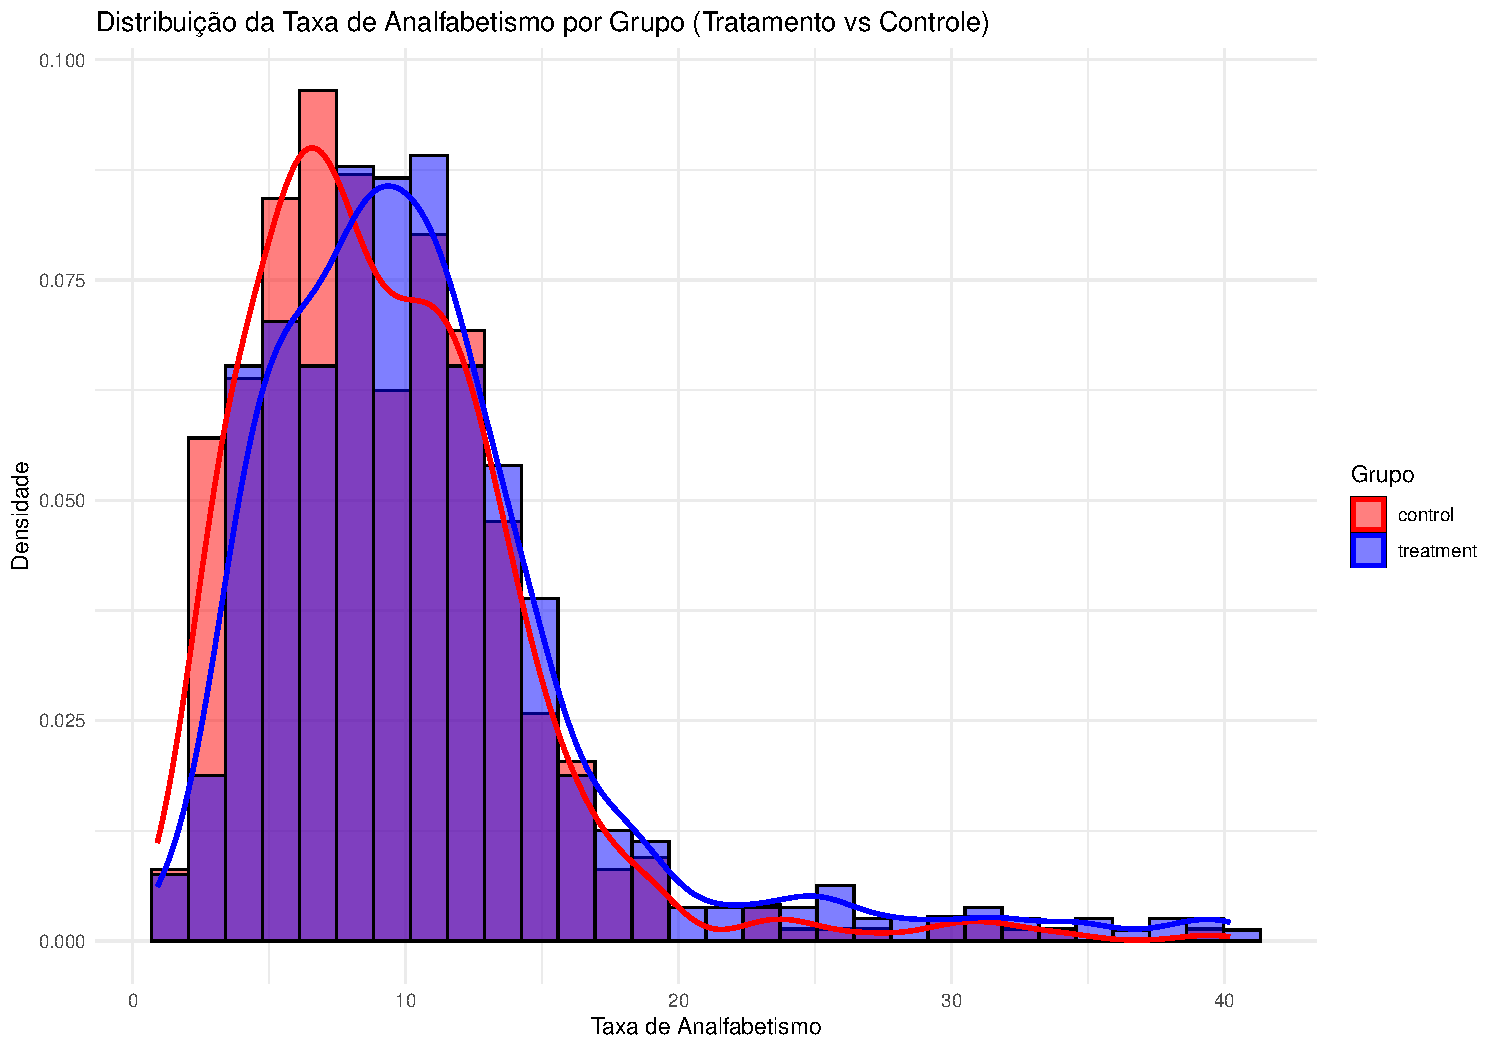
\includegraphics{graficos_files/figure-beamer/unnamed-chunk-9-1.pdf}
\end{frame}

\begin{frame}{Analfabetismo}
\phantomsection\label{analfabetismo-1}
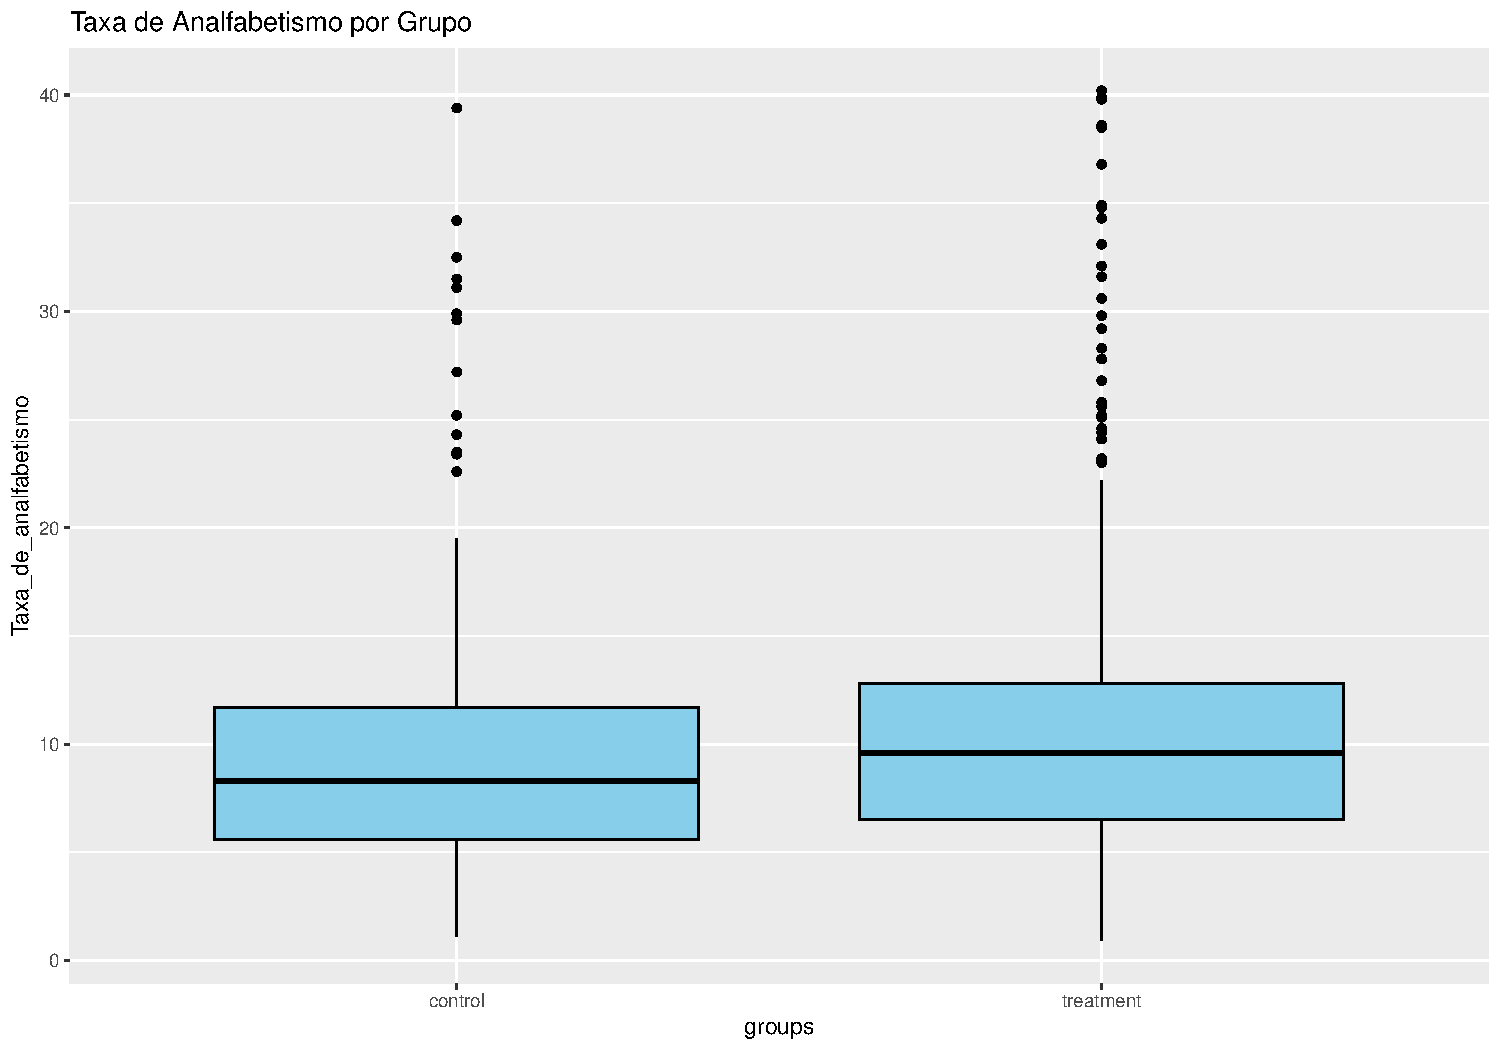
\includegraphics{graficos_files/figure-beamer/unnamed-chunk-10-1.pdf}
\end{frame}

\begin{frame}{Gini}
\phantomsection\label{gini}
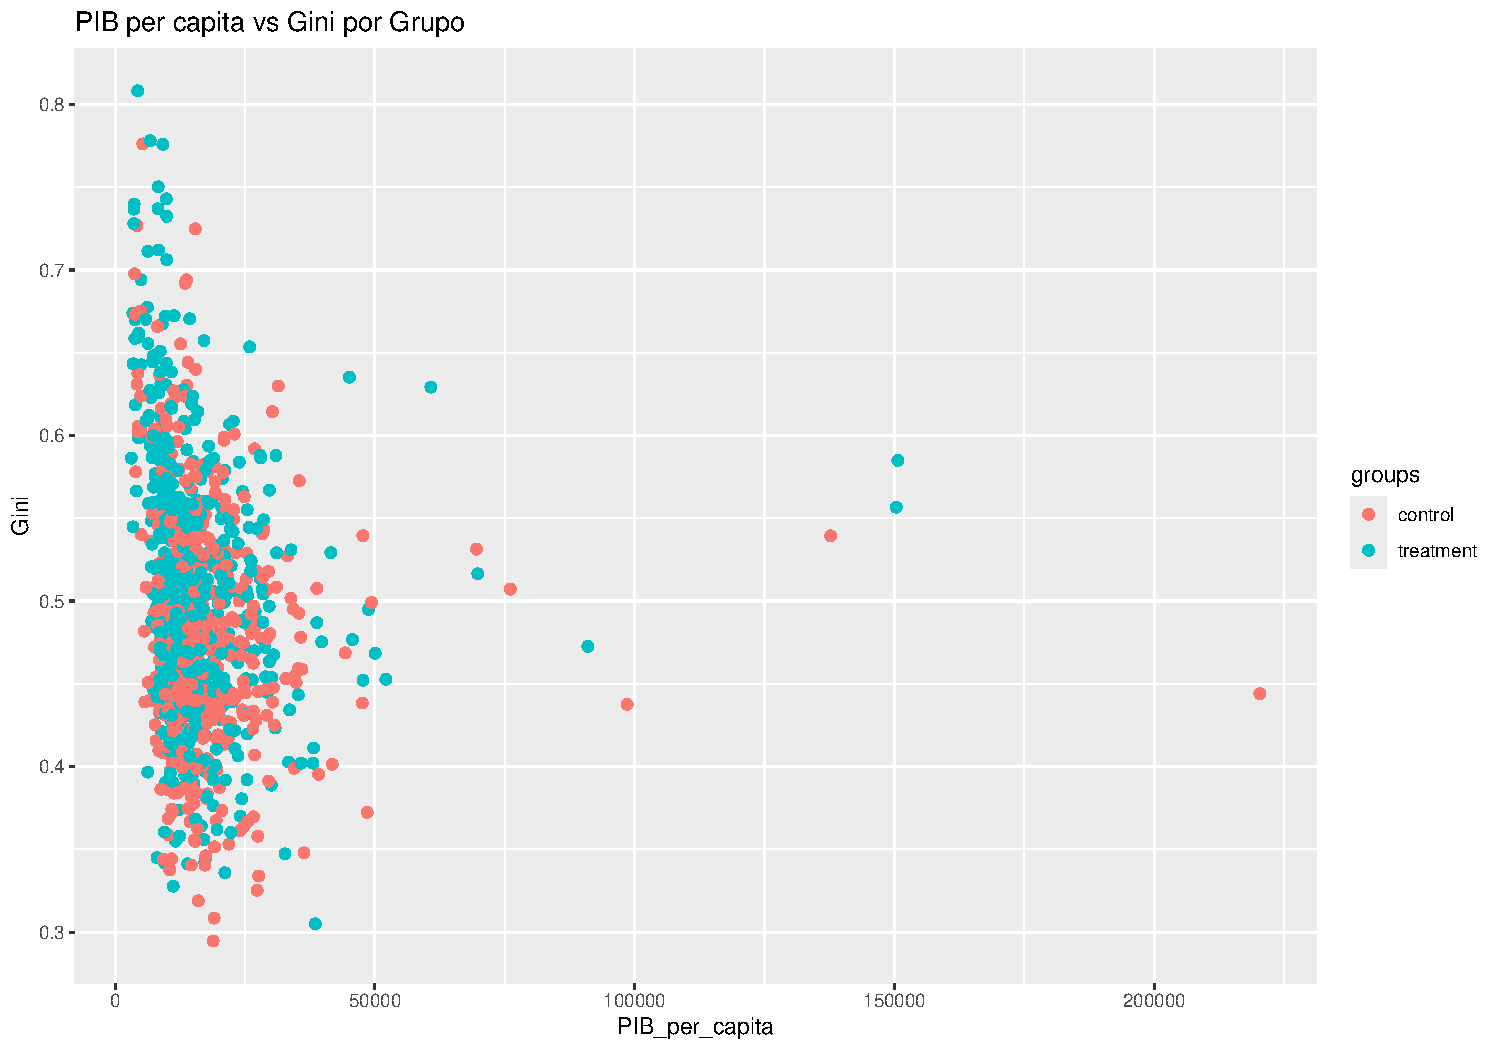
\includegraphics{graficos_files/figure-beamer/unnamed-chunk-11-1.pdf}
\end{frame}

\begin{frame}{Desemprego}
\phantomsection\label{desemprego}
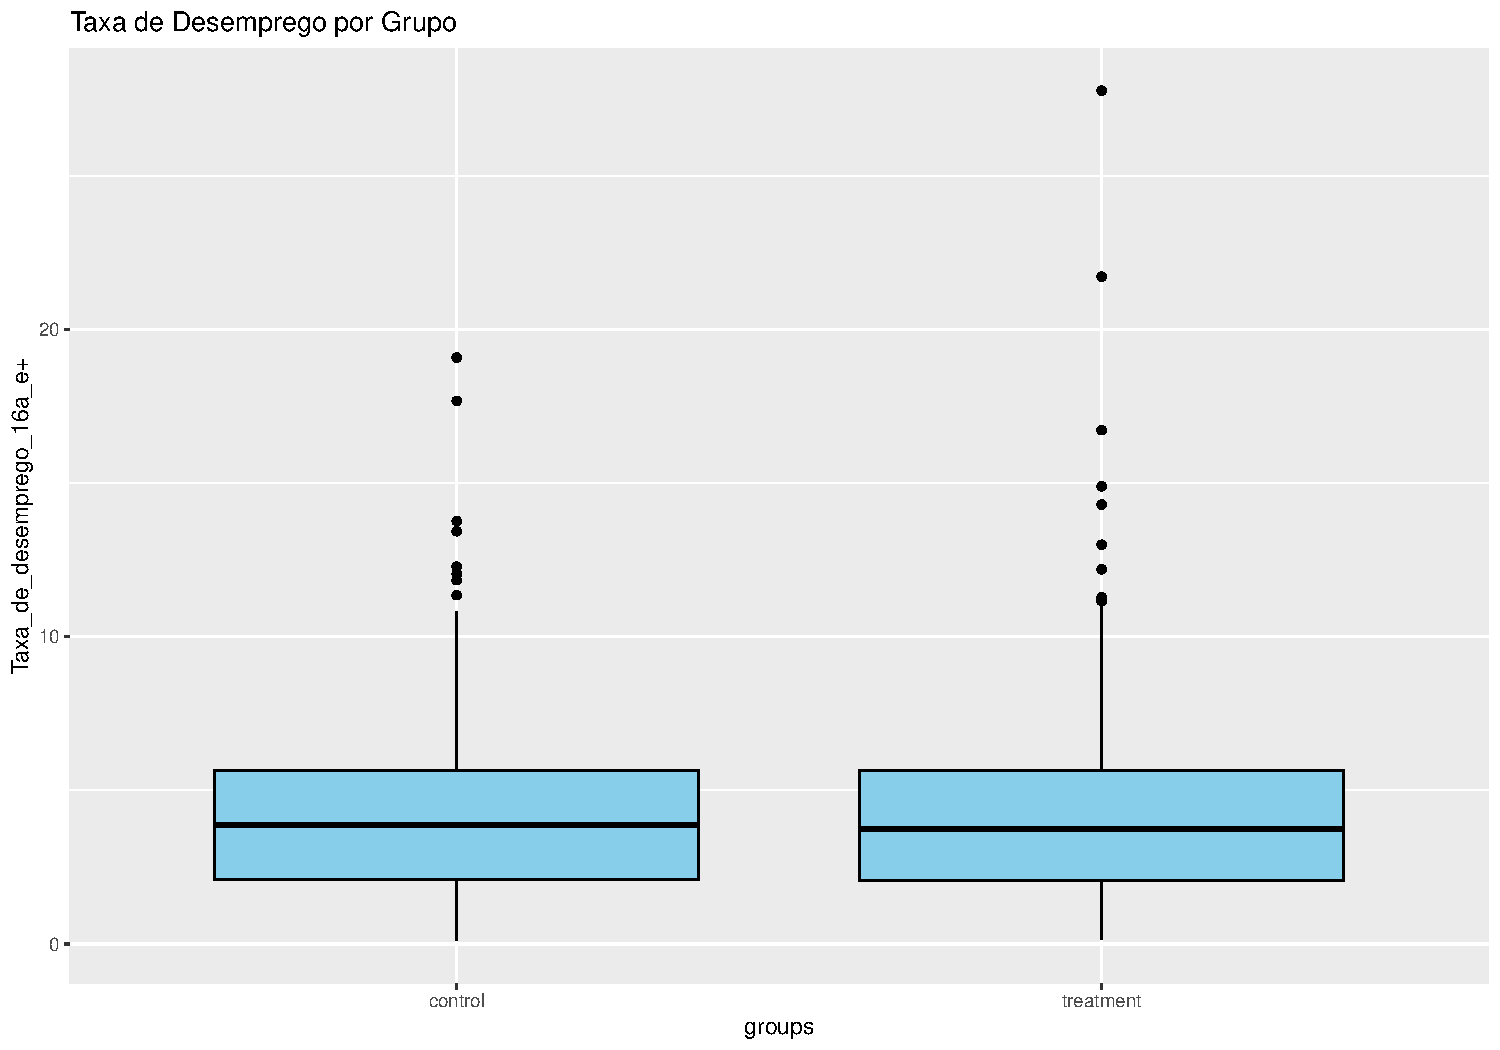
\includegraphics{graficos_files/figure-beamer/unnamed-chunk-12-1.pdf}
\end{frame}

\begin{frame}{Homicídios}
\phantomsection\label{homicuxeddios}
\begin{table}
\centering
\begin{tblr}[         %% tabularray outer open
]                     %% tabularray outer close
{                     %% tabularray inner open
colspec={Q[]Q[]Q[]Q[]Q[]Q[]Q[]Q[]Q[]},
column{1}={halign=l,},
column{2}={halign=l,},
column{3}={halign=l,},
column{4}={halign=l,},
column{5}={halign=l,},
column{6}={halign=l,},
column{7}={halign=l,},
column{8}={halign=l,},
column{9}={halign=l,},
}                     %% tabularray inner close
\toprule
& Unique & Missing Pct. & Mean & SD & Min & Median & Max & Histogram \\ \midrule %% TinyTableHeader
valor-2010 & 658 & 0 & 15.5 & 18.7 & 0.0 & 10.2 & 147.4 & 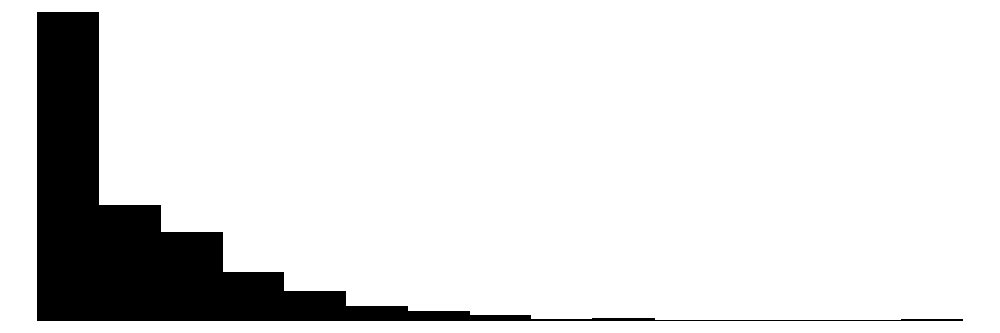
\includegraphics[height=1em]{tinytable_assets/idceg1t6zxpxpg7vludxre.png} \\
valor-2011 & 620 & 0 & 14.1 & 17.3 & 0.0 & 9.1 & 111.1 & 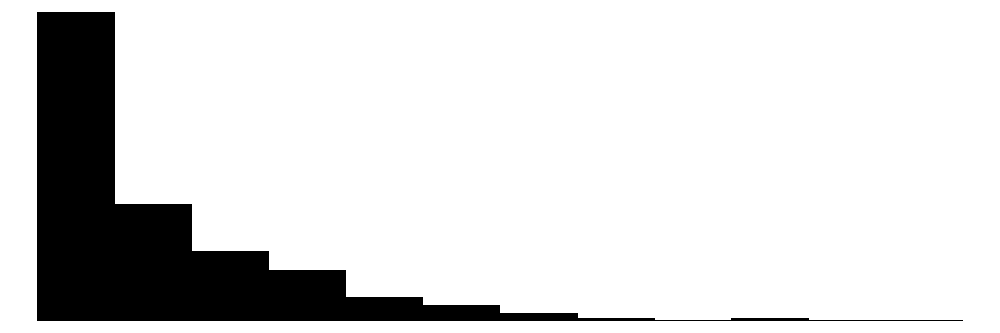
\includegraphics[height=1em]{tinytable_assets/idbbr5an3de969x2gk7t9w.png} \\
valor-2012 & 648 & 0 & 16.1 & 19.3 & 0.0 & 10.9 & 132.0 & 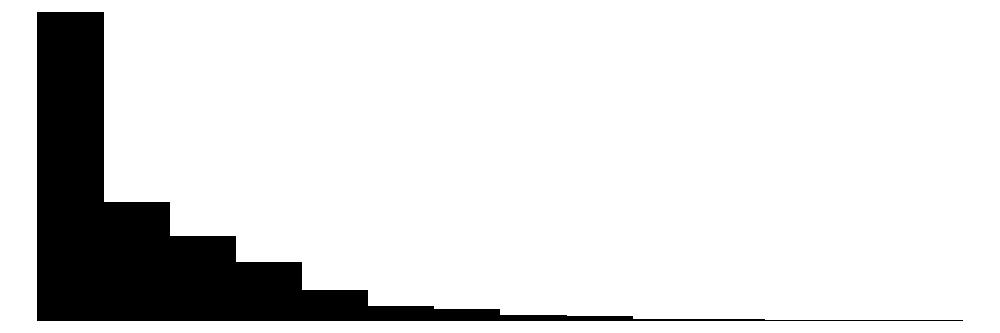
\includegraphics[height=1em]{tinytable_assets/id0wy4qyjpkp23gezgmziu.png} \\
valor-2013 & 662 & 0 & 15.9 & 19.8 & 0.0 & 11.7 & 183.7 & 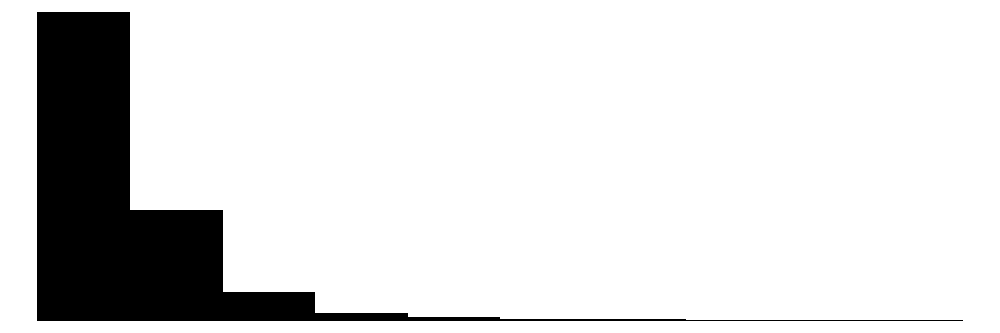
\includegraphics[height=1em]{tinytable_assets/idpv79m2hfdv29c2ha2hfn.png} \\
valor-2014 & 680 & 0 & 16.4 & 19.0 & 0.0 & 11.8 & 153.9 & 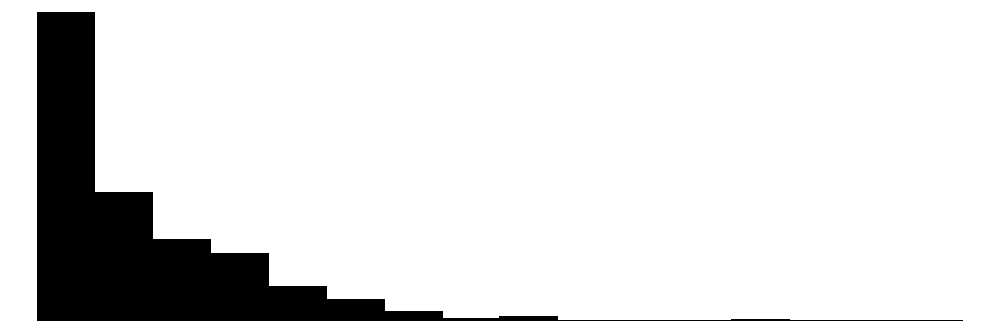
\includegraphics[height=1em]{tinytable_assets/idfejkiga8b3ykis1x05pt.png} \\
valor-2015 & 671 & 0 & 16.5 & 19.1 & 0.0 & 11.8 & 137.1 & 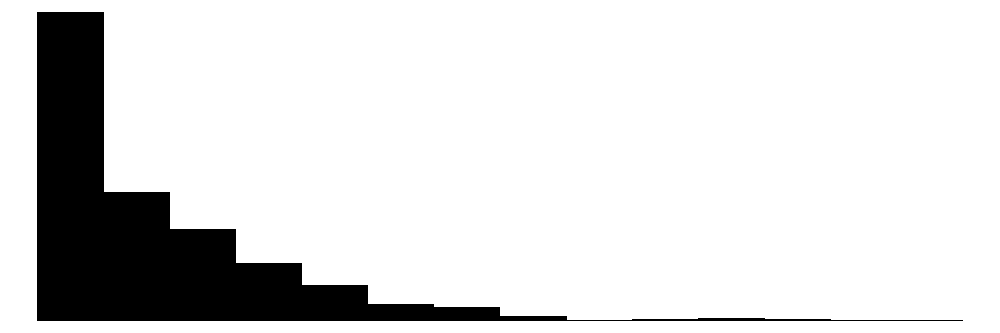
\includegraphics[height=1em]{tinytable_assets/idi18mhvchkqp9gnxerirw.png} \\
valor-2016 & 690 & 0 & 18.2 & 20.7 & 0.0 & 13.2 & 155.1 & 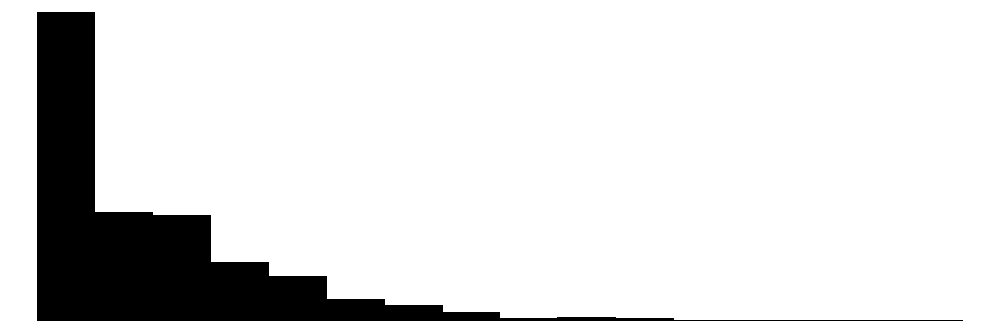
\includegraphics[height=1em]{tinytable_assets/id843nhfbinh7t0dhr5p1y.png} \\
valor-2017 & 706 & 0 & 19.6 & 22.2 & 0.0 & 14.6 & 222.0 & 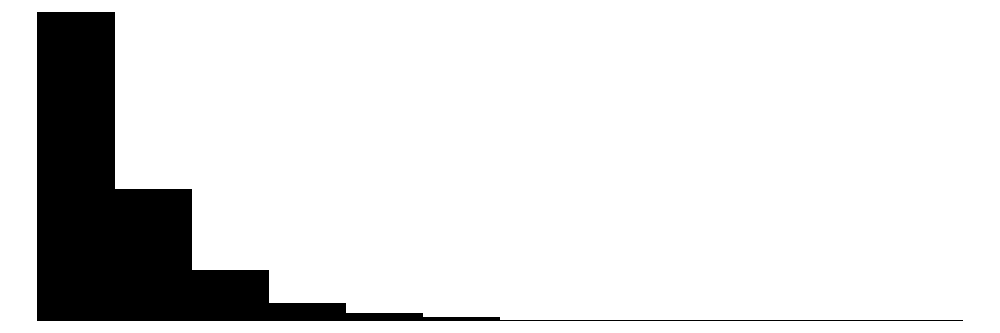
\includegraphics[height=1em]{tinytable_assets/idnb5hu1mknc1gj2zdit0j.png} \\
valor-2018 & 678 & 0 & 16.9 & 20.3 & 0.0 & 12.4 & 211.0 & 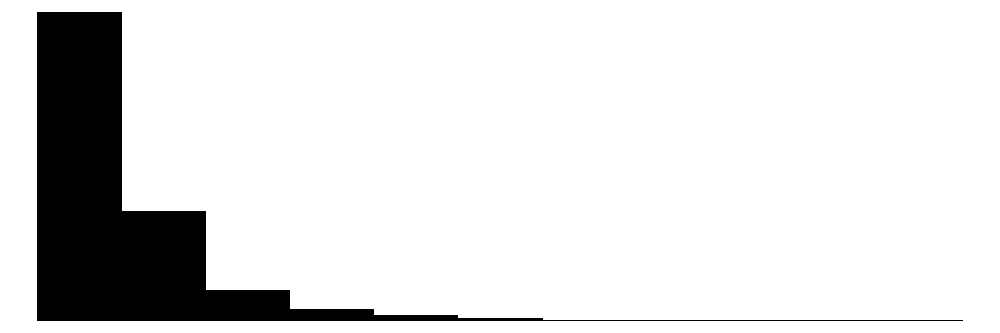
\includegraphics[height=1em]{tinytable_assets/idnr7pb63nc60zjo6j6baf.png} \\
valor-2019 & 657 & 0 & 15.5 & 19.2 & 0.0 & 10.9 & 176.7 & 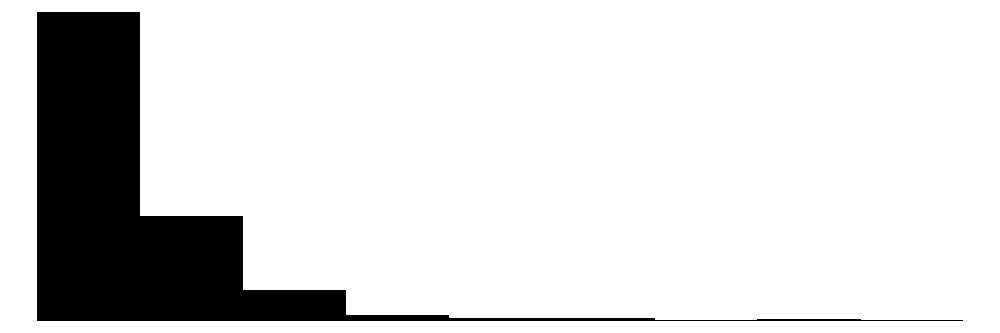
\includegraphics[height=1em]{tinytable_assets/ideqsln39qd1y567pl9ah0.png} \\
\bottomrule
\end{tblr}
\end{table}
\end{frame}

\begin{frame}{Homicídios}
\phantomsection\label{homicuxeddios-1}
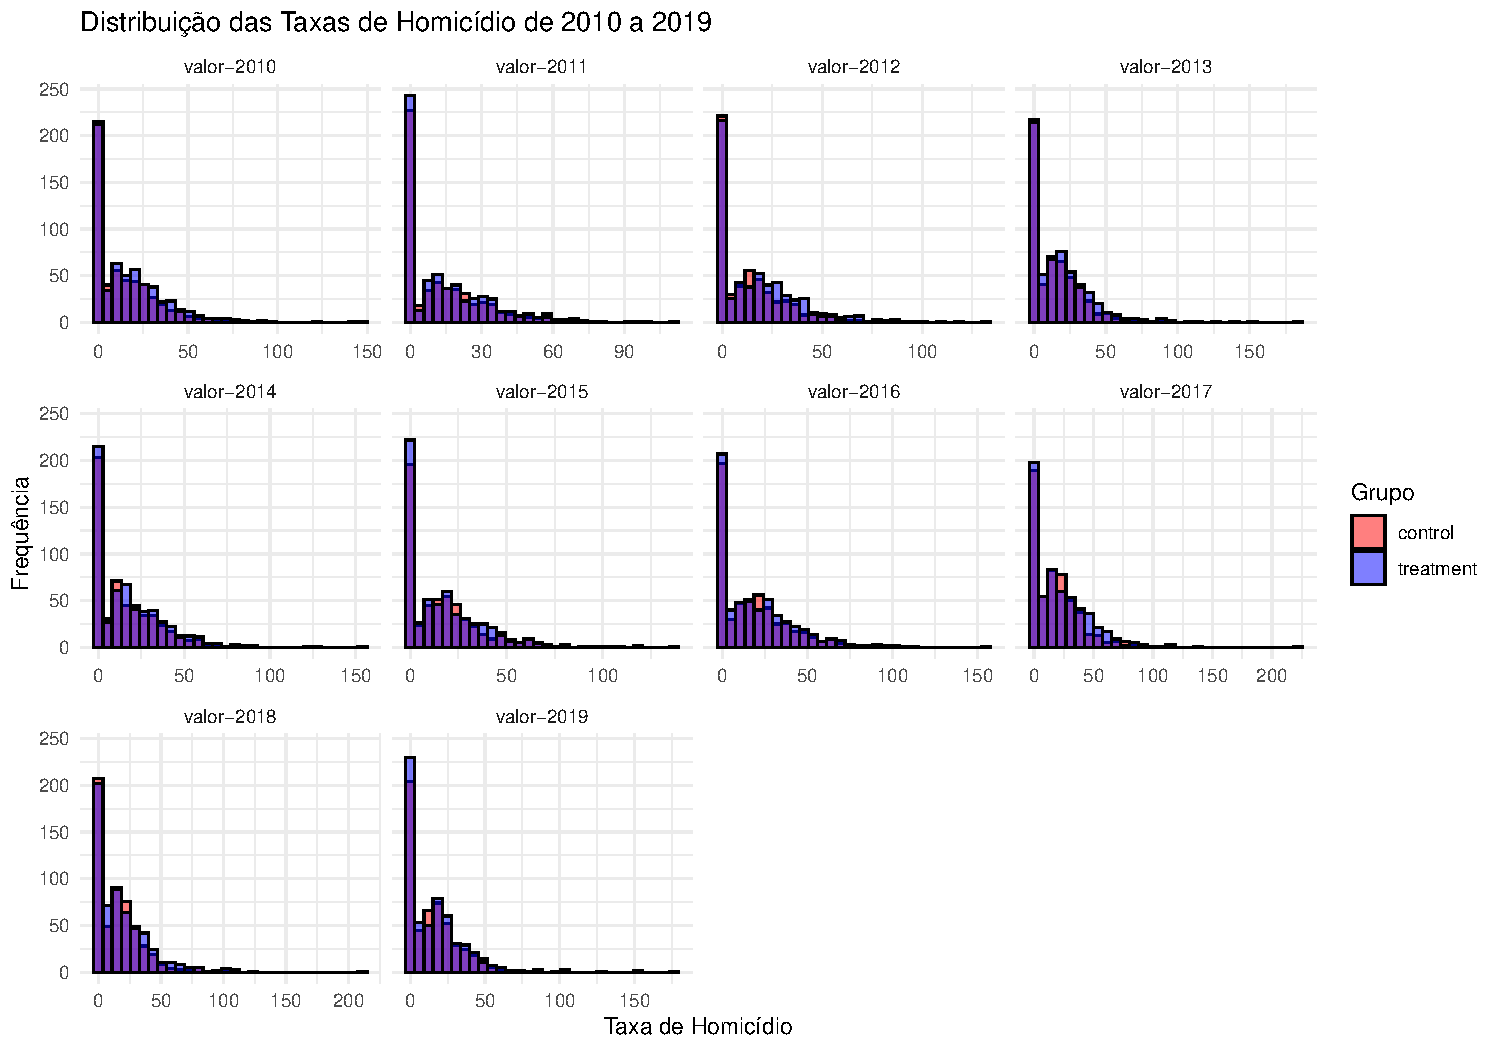
\includegraphics{graficos_files/figure-beamer/unnamed-chunk-14-1.pdf}
\end{frame}

\begin{frame}{Homicídios}
\phantomsection\label{homicuxeddios-2}
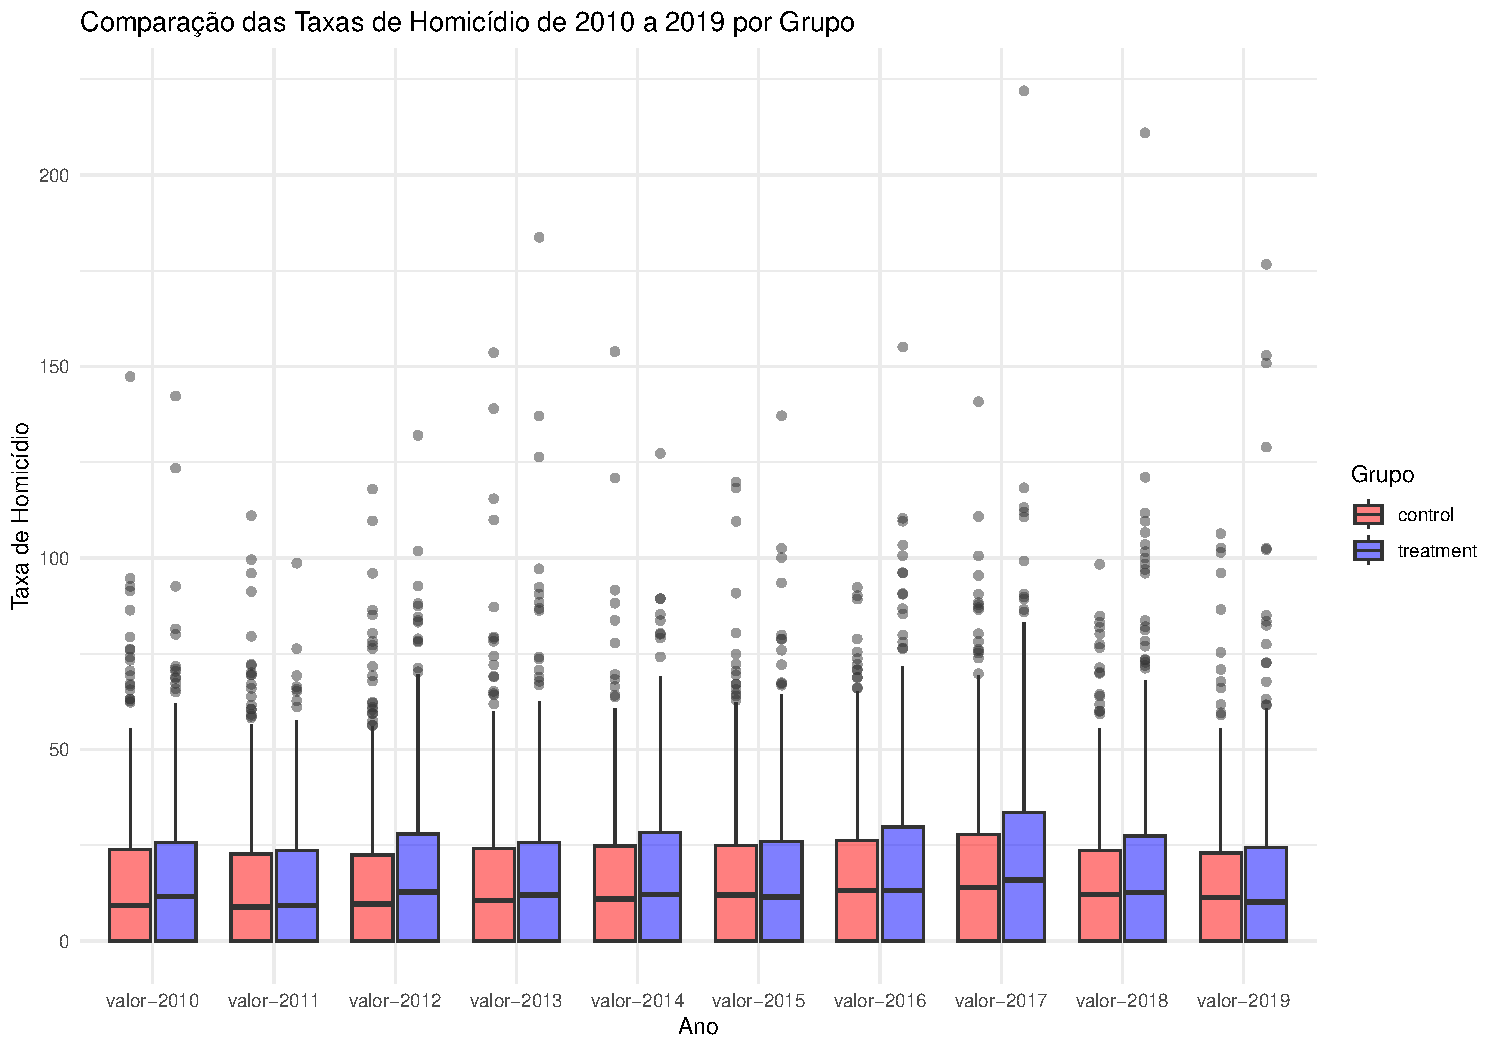
\includegraphics{graficos_files/figure-beamer/unnamed-chunk-15-1.pdf}
\end{frame}

\begin{frame}{Homicídios}
\phantomsection\label{homicuxeddios-3}
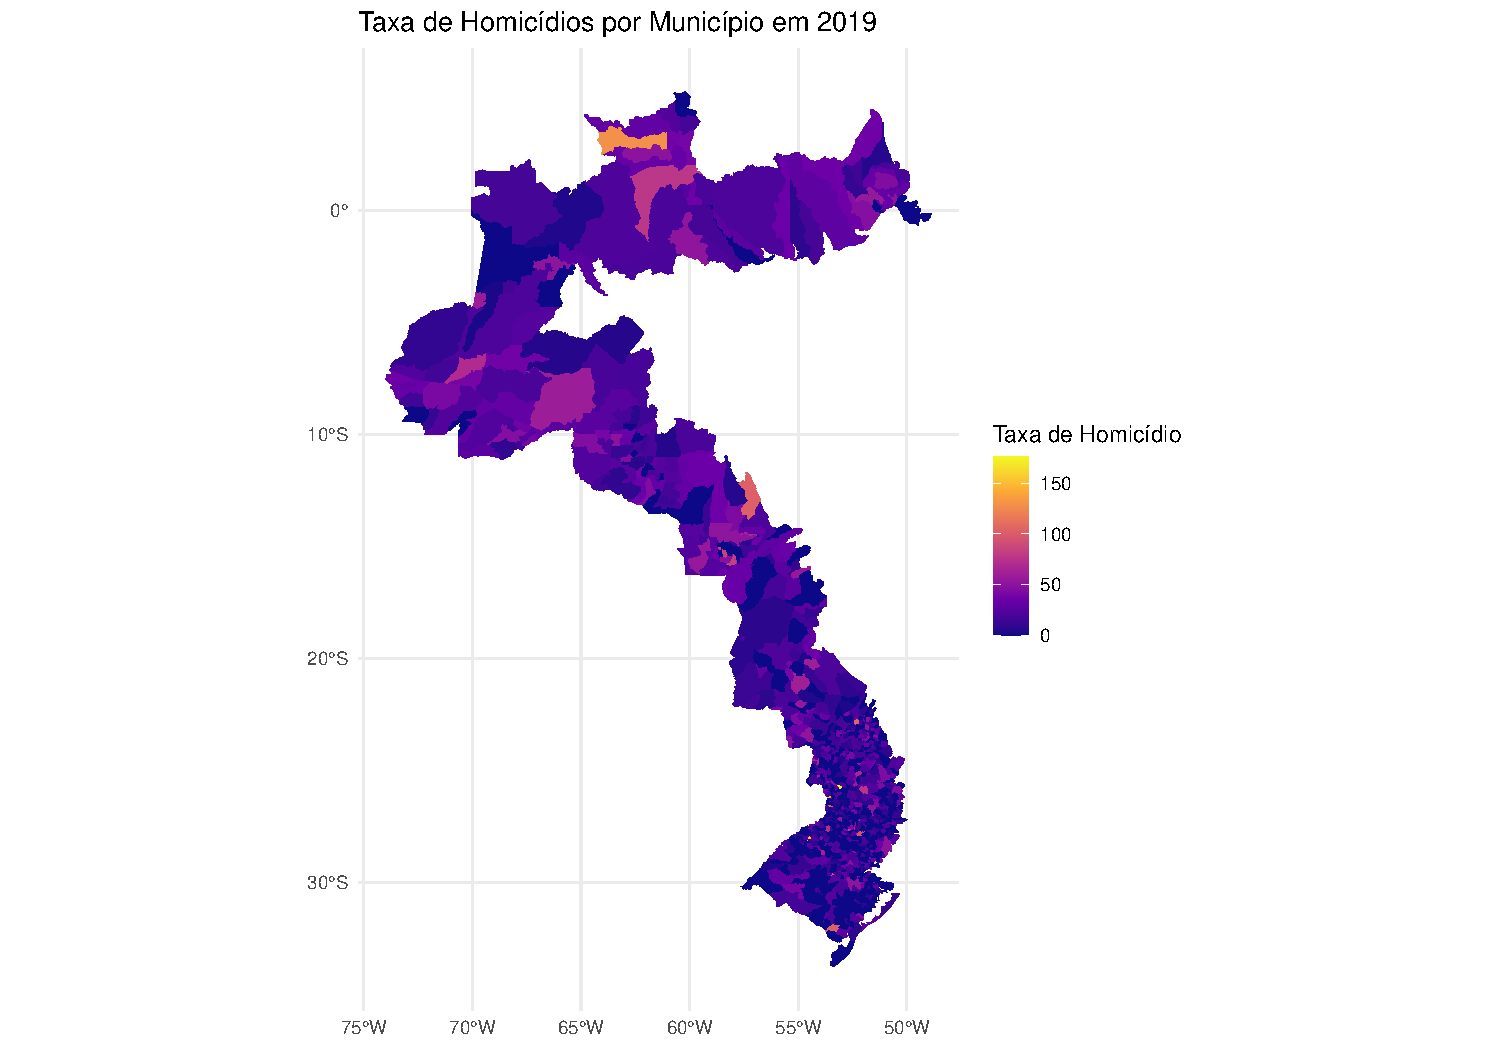
\includegraphics{graficos_files/figure-beamer/unnamed-chunk-16-1.pdf}
\end{frame}

\begin{frame}{Outros crimes}
\phantomsection\label{outros-crimes}
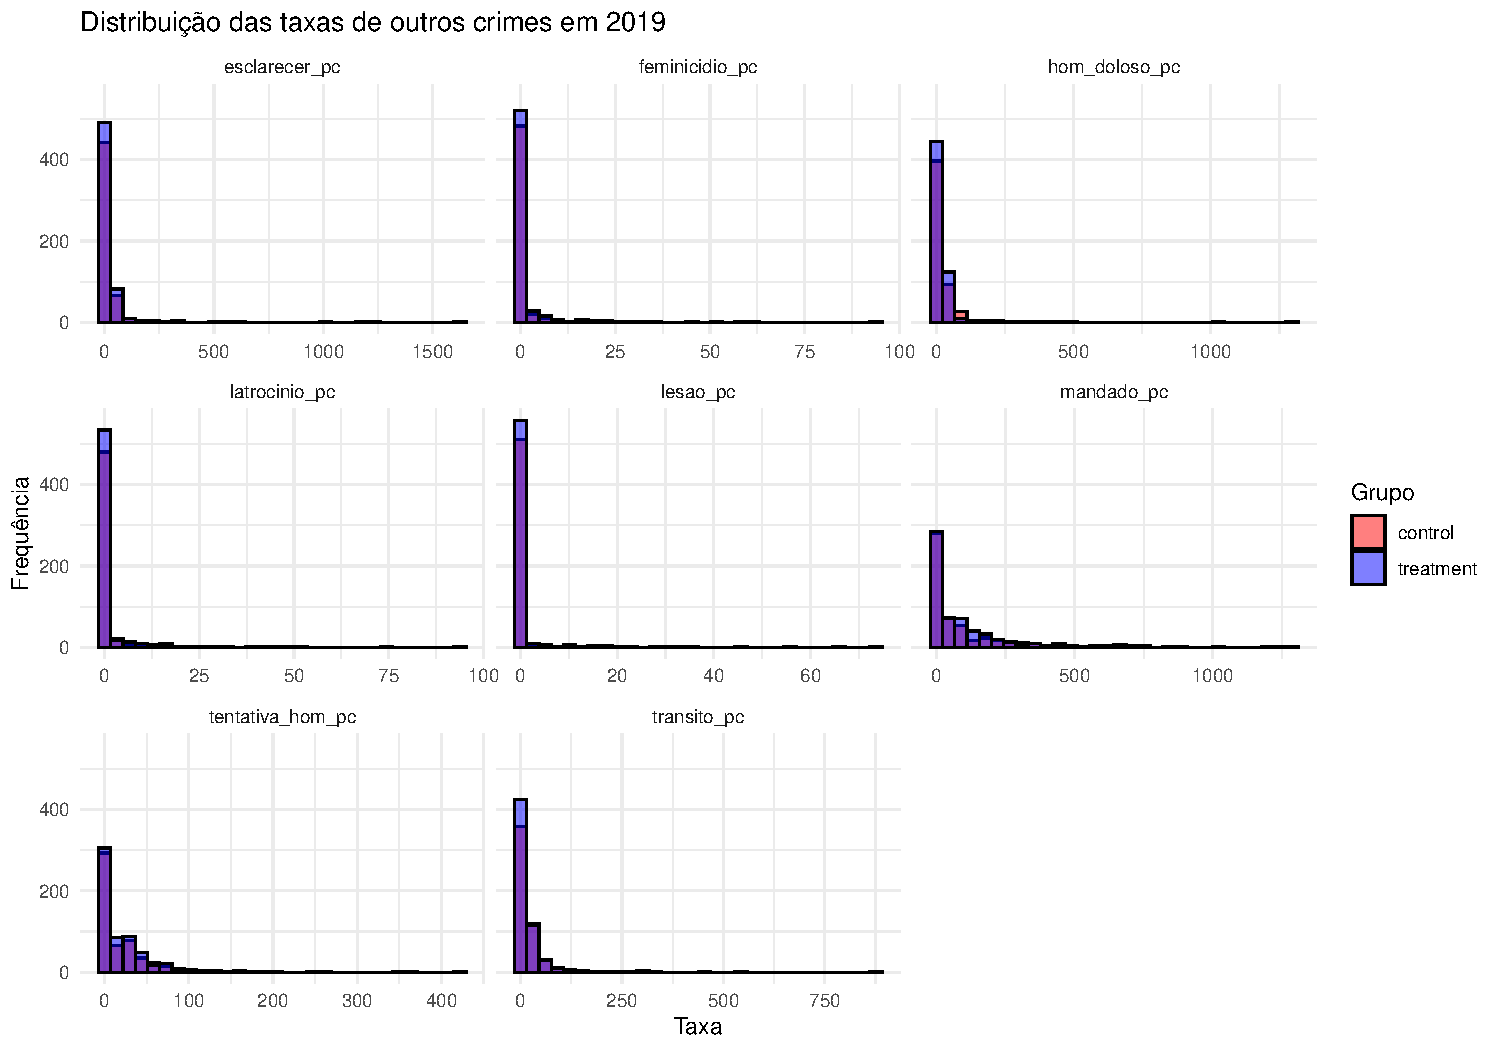
\includegraphics{graficos_files/figure-beamer/unnamed-chunk-17-1.pdf}
\end{frame}

\begin{frame}{Outros crimes}
\phantomsection\label{outros-crimes-1}
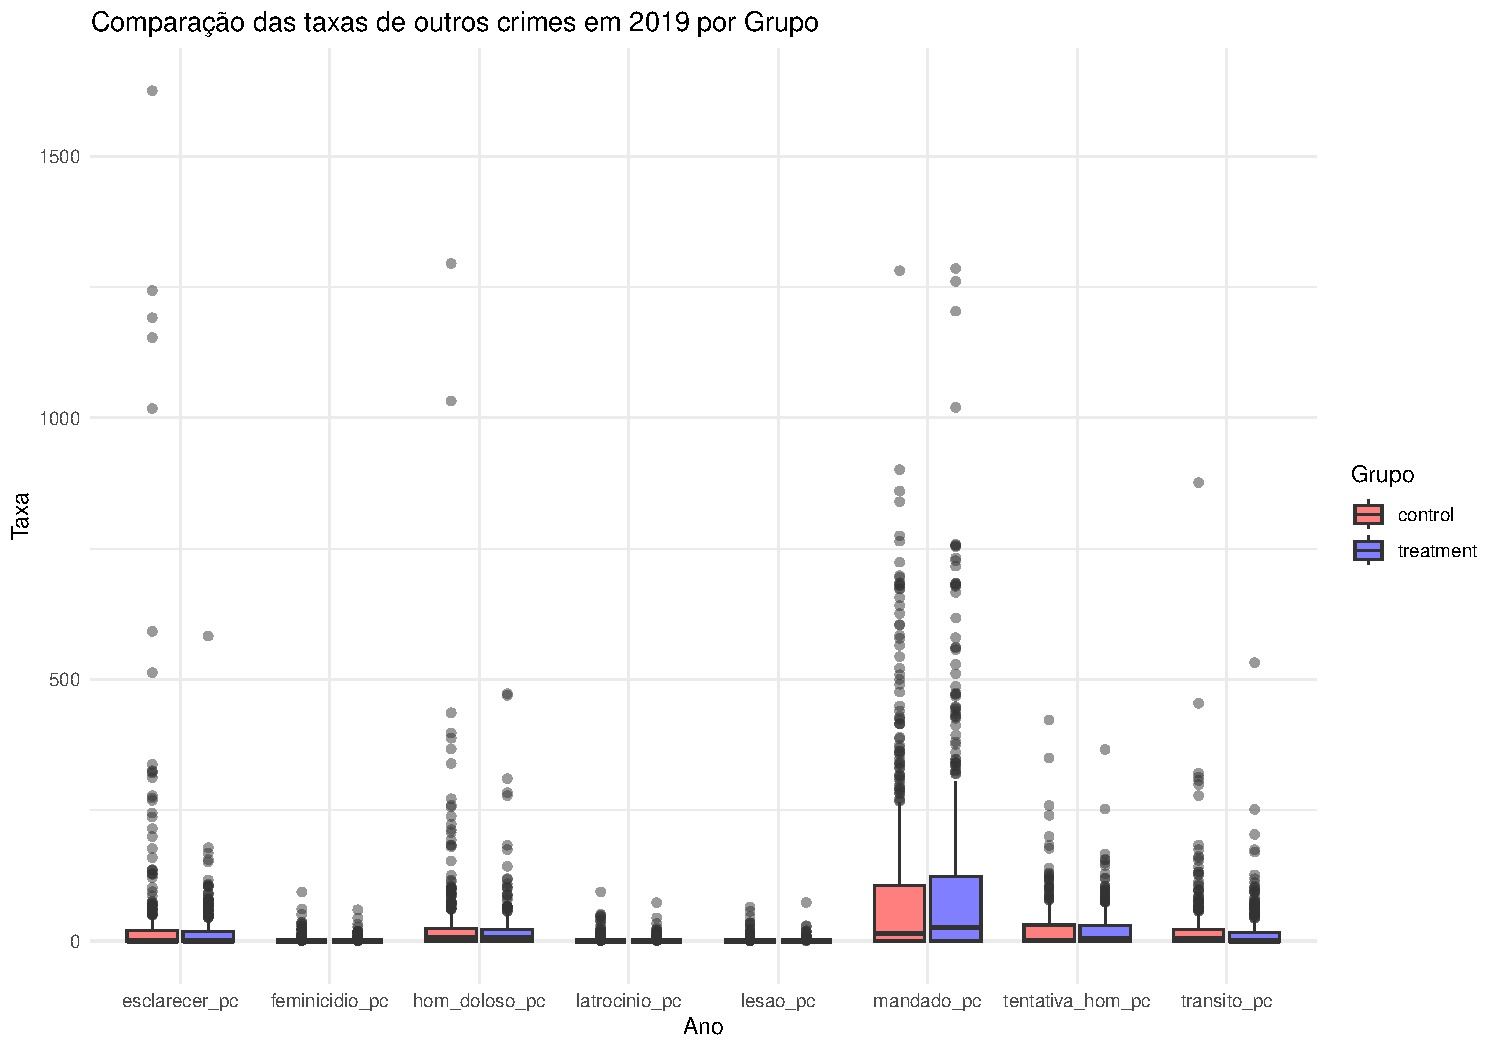
\includegraphics{graficos_files/figure-beamer/unnamed-chunk-18-1.pdf}
\end{frame}

\begin{frame}{Feminicídios}
\phantomsection\label{feminicuxeddios}
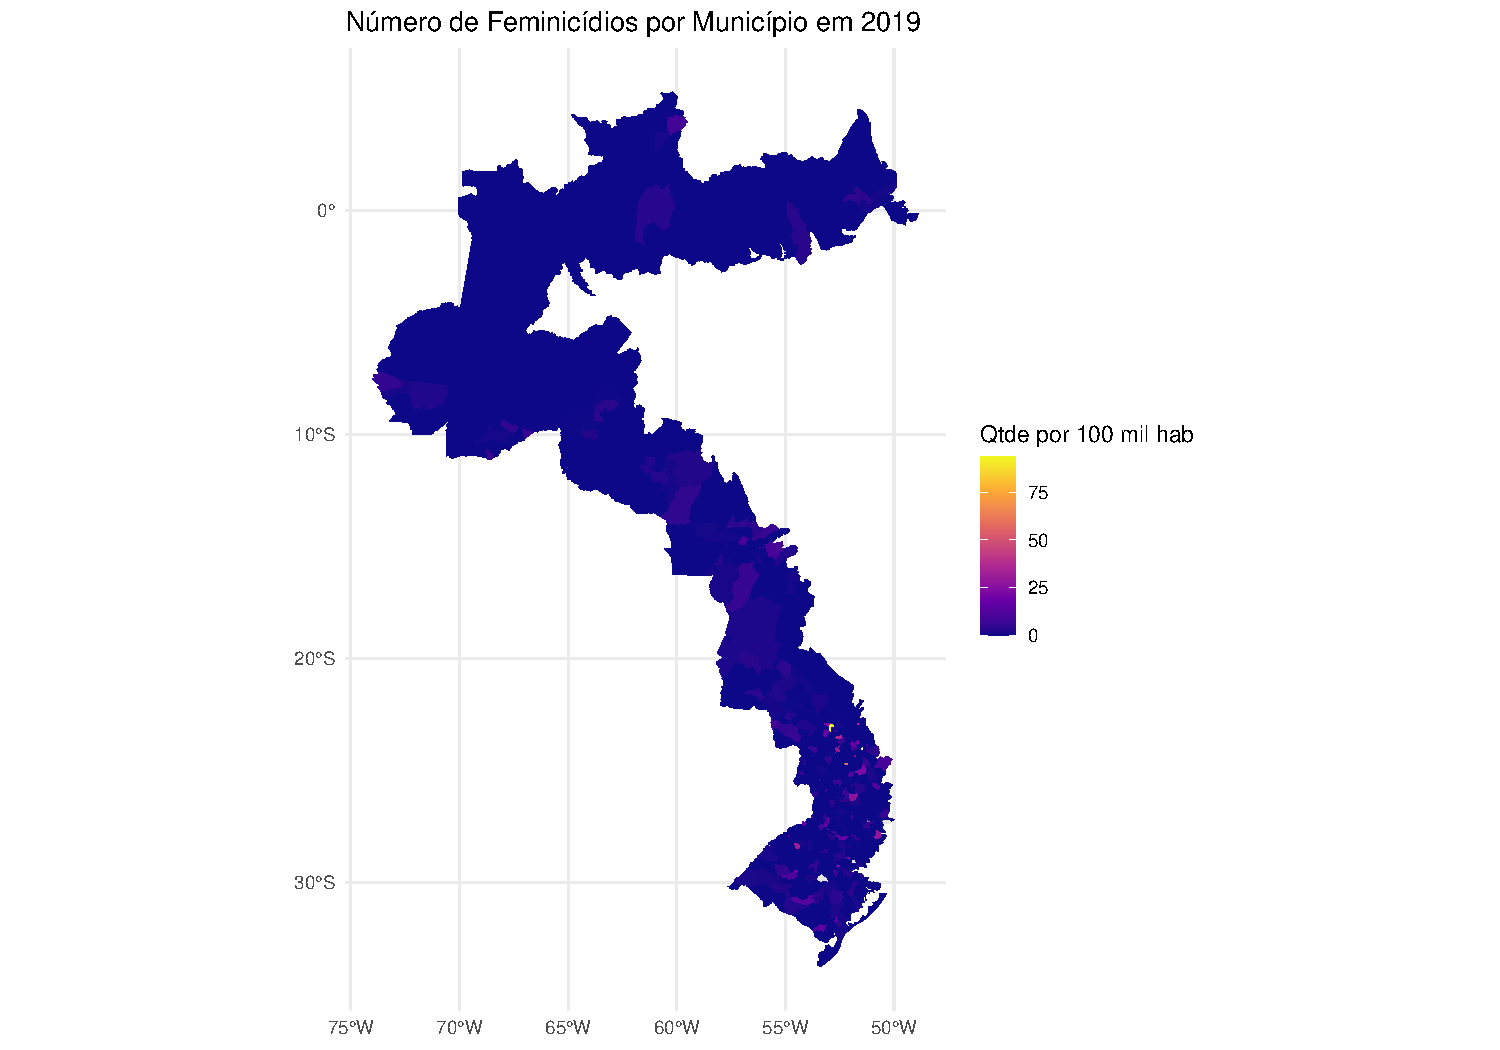
\includegraphics{graficos_files/figure-beamer/unnamed-chunk-19-1.pdf}
\end{frame}

\begin{frame}{Homicídio doloso}
\phantomsection\label{homicuxeddio-doloso}
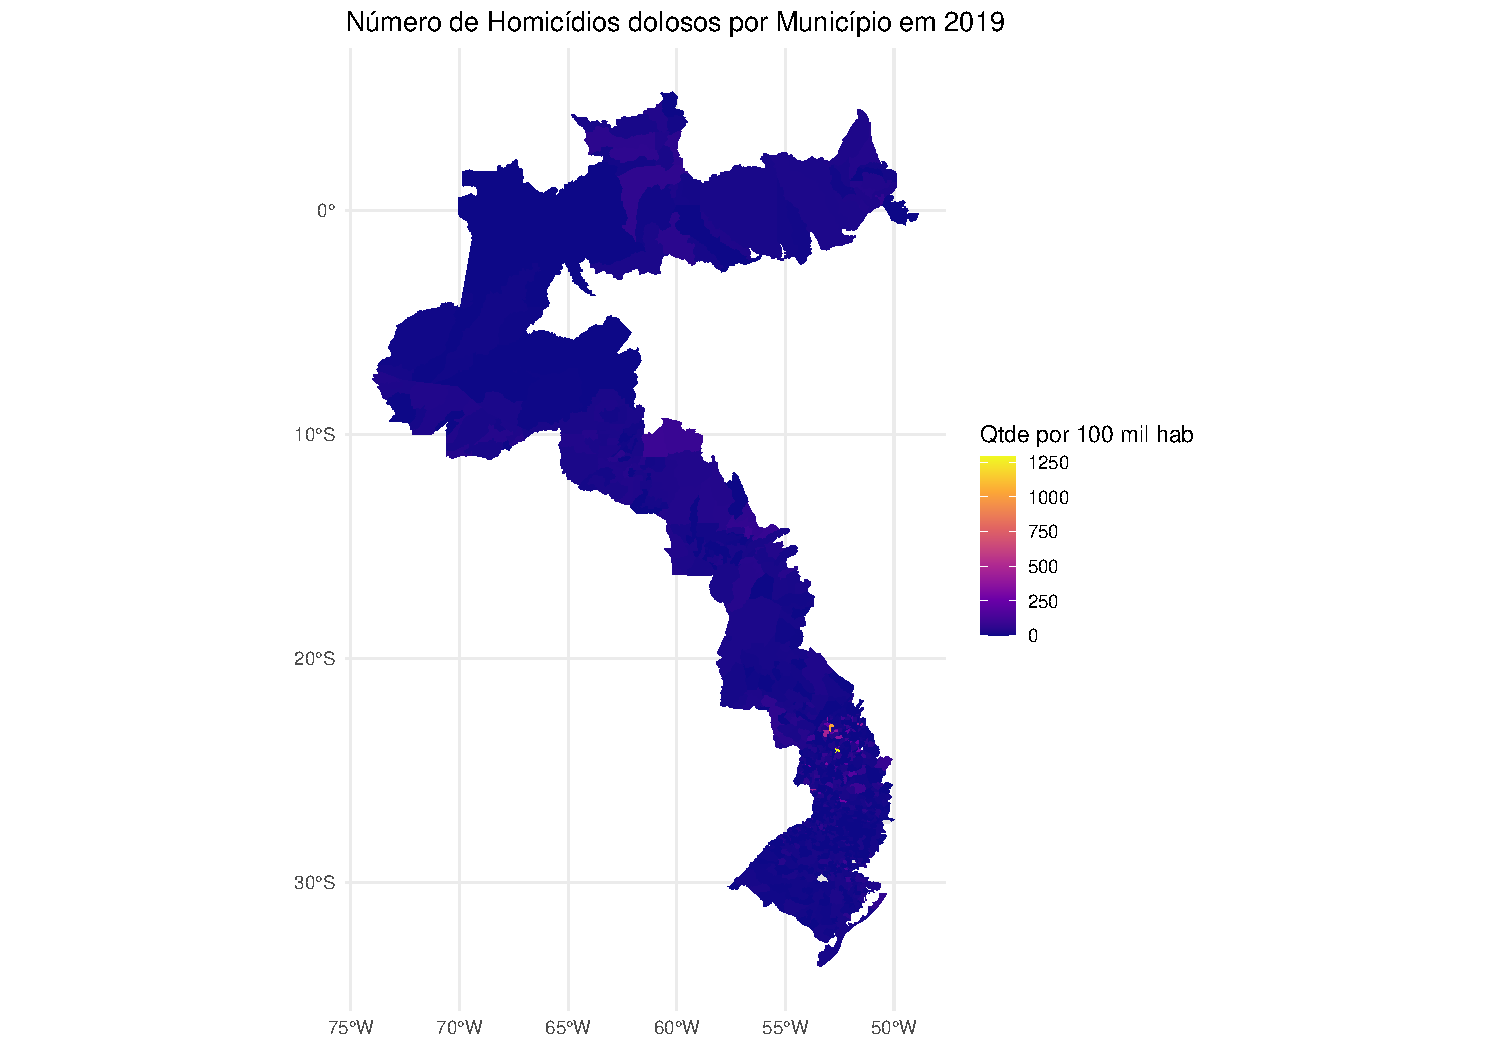
\includegraphics{graficos_files/figure-beamer/unnamed-chunk-20-1.pdf}
\end{frame}

\begin{frame}{Lesão seguida de morte}
\phantomsection\label{lesuxe3o-seguida-de-morte}
\includegraphics{graficos_files/figure-beamer/unnamed-chunk-21-1.pdf}
\end{frame}

\begin{frame}{Mandados de prisão}
\phantomsection\label{mandados-de-prisuxe3o}
\includegraphics{graficos_files/figure-beamer/unnamed-chunk-22-1.pdf}
\end{frame}

\begin{frame}{Mortes no trânsito}
\phantomsection\label{mortes-no-truxe2nsito}
\includegraphics{graficos_files/figure-beamer/unnamed-chunk-23-1.pdf}
\end{frame}

\begin{frame}{Mortes a esclarecer}
\phantomsection\label{mortes-a-esclarecer}
\includegraphics{graficos_files/figure-beamer/unnamed-chunk-24-1.pdf}
\end{frame}

\begin{frame}{Latrocínio}
\phantomsection\label{latrocuxednio}
\includegraphics{graficos_files/figure-beamer/unnamed-chunk-25-1.pdf}
\end{frame}

\begin{frame}{Tentativa de homicídio}
\phantomsection\label{tentativa-de-homicuxeddio}
\includegraphics{graficos_files/figure-beamer/unnamed-chunk-26-1.pdf}
\end{frame}

\begin{frame}{Regressões: Homicídios X grupos}
\phantomsection\label{regressuxf5es-homicuxeddios-x-grupos}
\begin{table}
\centering
\begin{talltblr}[         %% tabularray outer open
entry=none,label=none,
note{}={+ p < 0.1, * p < 0.05, ** p < 0.01, *** p < 0.001},
]                     %% tabularray outer close
{                     %% tabularray inner open
colspec={Q[]Q[]Q[]Q[]Q[]Q[]},
column{1}={halign=l,},
column{2}={halign=c,},
column{3}={halign=c,},
column{4}={halign=c,},
column{5}={halign=c,},
column{6}={halign=c,},
hline{6}={1,2,3,4,5,6}{solid, 0.05em, black},
}                     %% tabularray inner close
\toprule
& hom 2010 & hom 2011 & hom 2012 & hom 2013 & hom 2014 \\ \midrule %% TinyTableHeader
(Intercept) & 14.846*** & 14.421*** & 14.746*** & 15.193*** & 15.781*** \\
& (0.803)   & (0.742)   & (0.828)   & (0.848)   & (0.817)   \\
treatedTRUE & 1.316     & -0.639    & 2.585*    & 1.399     & 1.278     \\
& (1.113)   & (1.029)   & (1.149)   & (1.176)   & (1.133)   \\
Num.Obs.    & 1131      & 1131      & 1131      & 1131      & 1131      \\
R2          & 0.001     & 0.000     & 0.004     & 0.001     & 0.001     \\
R2 Adj.     & 0.000     & -0.001    & 0.004     & 0.000     & 0.000     \\
AIC         & 9838.1    & 9660.2    & 9909.7    & 9962.9    & 9878.1    \\
BIC         & 9853.2    & 9675.3    & 9924.8    & 9978.0    & 9893.1    \\
Log.Lik.    & -4916.065 & -4827.090 & -4951.850 & -4978.457 & -4936.027 \\
F           & 1.398     & 0.386     & 5.064     & 1.415     & 1.272     \\
RMSE        & 18.68     & 17.27     & 19.29     & 19.74     & 19.02     \\
\bottomrule
\end{talltblr}
\end{table}
\end{frame}

\begin{frame}{Outros crimes X grupos}
\phantomsection\label{outros-crimes-x-grupos}
\begin{table}
\centering
\begin{tblr}[         %% tabularray outer open
]                     %% tabularray outer close
{                     %% tabularray inner open
colspec={Q[]Q[]Q[]Q[]Q[]},
column{1}={halign=l,},
column{2}={halign=c,},
column{3}={halign=c,},
column{4}={halign=c,},
column{5}={halign=c,},
hline{6}={1,2,3,4,5}{solid, 0.05em, black},
}                     %% tabularray inner close
\toprule
& (1) & (2) & (3) & (4) \\ \midrule %% TinyTableHeader
(Intercept) & 1.731     & 47.017    & 1.283     & 96.853    \\
& (0.281)   & (11.316)  & (0.298)   & (7.474)   \\
treatedTRUE & -0.676    & -29.496   & -0.728    & 3.194     \\
& (0.389)   & (15.680)  & (0.413)   & (10.356)  \\
Num.Obs.    & 1129      & 1129      & 1129      & 1129      \\
R2          & 0.003     & 0.003     & 0.003     & 0.000     \\
R2 Adj.     & 0.002     & 0.002     & 0.002     & -0.001    \\
AIC         & 7445.1    & 15791.6   & 7577.5    & 14854.9   \\
BIC         & 7460.2    & 15806.7   & 7592.6    & 14870.0   \\
Log.Lik.    & -3719.538 & -7892.809 & -3785.752 & -7424.470 \\
F           & 3.018     & 3.539     & 3.115     & 0.095     \\
RMSE        & 6.52      & 262.97    & 6.92      & 173.68    \\
\bottomrule
\end{tblr}
\end{table}
\end{frame}

\begin{frame}{Outros crimes X grupos}
\phantomsection\label{outros-crimes-x-grupos-1}
\begin{table}
\centering
\begin{tblr}[         %% tabularray outer open
]                     %% tabularray outer close
{                     %% tabularray inner open
colspec={Q[]Q[]Q[]Q[]Q[]},
column{1}={halign=l,},
column{2}={halign=c,},
column{3}={halign=c,},
column{4}={halign=c,},
column{5}={halign=c,},
hline{6}={1,2,3,4,5}{solid, 0.05em, black},
}                     %% tabularray inner close
\toprule
& (1) & (2) & (3) & (4) \\ \midrule %% TinyTableHeader
(Intercept) & 26.453    & 106.648   & 2.423     & 34.612    \\
& (3.715)   & (47.100)  & (0.488)   & (7.073)   \\
treatedTRUE & -12.133   & -92.666   & -1.463    & -15.081   \\
& (5.148)   & (65.264)  & (0.676)   & (9.800)   \\
Num.Obs.    & 1129      & 1129      & 1129      & 1129      \\
R2          & 0.005     & 0.002     & 0.004     & 0.002     \\
R2 Adj.     & 0.004     & 0.001     & 0.003     & 0.001     \\
AIC         & 13276.8   & 19011.6   & 8692.1    & 14730.4   \\
BIC         & 13291.9   & 19026.7   & 8707.1    & 14745.5   \\
Log.Lik.    & -6635.416 & -9502.822 & -4343.028 & -7362.190 \\
F           & 5.554     & 2.016     & 4.685     & 2.368     \\
RMSE        & 86.34     & 1094.54   & 11.33     & 164.36    \\
\bottomrule
\end{tblr}
\end{table}
\end{frame}

\begin{frame}{Outros crimes X grupos e arcos}
\phantomsection\label{outros-crimes-x-grupos-e-arcos}
\begin{table}
\centering
\begin{tblr}[         %% tabularray outer open
]                     %% tabularray outer close
{                     %% tabularray inner open
colspec={Q[]Q[]Q[]Q[]Q[]},
column{1}={halign=l,},
column{2}={halign=c,},
column{3}={halign=c,},
column{4}={halign=c,},
column{5}={halign=c,},
hline{14}={1,2,3,4,5}{solid, 0.05em, black},
}                     %% tabularray inner close
\toprule
& (1) & (2) & (3) & (4) \\ \midrule %% TinyTableHeader
(Intercept)                   & 0.695     & 23.622    & 0.437     & 113.337   \\
& (0.763)   & (30.796)  & (0.810)   & (19.850)  \\
treatedTRUE                   & -0.058    & -5.012    & 0.227     & 22.171    \\
& (1.004)   & (40.537)  & (1.066)   & (26.129)  \\
arcosArco Norte               & -0.249    & -7.537    & 0.580     & -50.960   \\
& (1.593)   & (64.331)  & (1.692)   & (41.465)  \\
arcosArco Sul                 & 1.326     & 30.061    & 1.039     & -24.504   \\
& (0.825)   & (33.324)  & (0.877)   & (21.479)  \\
treatedTRUE × arcosArco Norte & 0.273     & 5.654     & -0.722    & 9.725     \\
& (1.895)   & (76.488)  & (2.012)   & (49.301)  \\
treatedTRUE × arcosArco Sul   & -0.741    & -31.281   & -1.171    & -18.572   \\
& (1.100)   & (44.421)  & (1.169)   & (28.632)  \\
Num.Obs.                      & 1117      & 1117      & 1117      & 1117      \\
R2                            & 0.007     & 0.004     & 0.004     & 0.007     \\
R2 Adj.                       & 0.002     & 0.000     & 0.000     & 0.003     \\
AIC                           & 7380.6    & 15642.3   & 7515.1    & 14661.2   \\
BIC                           & 7415.8    & 15677.4   & 7550.2    & 14696.3   \\
Log.Lik.                      & -3683.317 & -7814.158 & -3750.531 & -7323.582 \\
F                             & 1.549     & 0.963     & 0.953     & 1.595     \\
RMSE                          & 6.54      & 264.21    & 6.95      & 170.30    \\
\bottomrule
\end{tblr}
\end{table}
\end{frame}

\begin{frame}{Outros crimes X grupos e arcos}
\phantomsection\label{outros-crimes-x-grupos-e-arcos-1}
\begin{table}
\centering
\begin{tblr}[         %% tabularray outer open
]                     %% tabularray outer close
{                     %% tabularray inner open
colspec={Q[]Q[]Q[]Q[]Q[]},
column{1}={halign=l,},
column{2}={halign=c,},
column{3}={halign=c,},
column{4}={halign=c,},
column{5}={halign=c,},
hline{14}={1,2,3,4,5}{solid, 0.05em, black},
}                     %% tabularray inner close
\toprule
& (1) & (2) & (3) & (4) \\ \midrule %% TinyTableHeader
(Intercept)                   & 15.870    & 18.085    & 0.957     & 36.823    \\
& (10.097)  & (128.207) & (1.327)   & (19.247)  \\
treatedTRUE                   & -4.478    & 2.060     & -0.290    & -5.899    \\
& (13.291)  & (168.761) & (1.746)   & (25.335)  \\
arcosArco Norte               & -10.497   & -16.919   & -0.132    & -25.355   \\
& (21.092)  & (267.816) & (2.771)   & (40.205)  \\
arcosArco Sul                 & 13.895    & 111.848   & 1.856     & -0.623    \\
& (10.926)  & (138.731) & (1.435)   & (20.827)  \\
treatedTRUE × arcosArco Norte & 6.614     & -1.891    & 0.799     & 5.252     \\
& (25.078)  & (318.429) & (3.295)   & (47.803)  \\
treatedTRUE × arcosArco Sul   & -9.134    & -117.413  & -1.555    & -12.085   \\
& (14.564)  & (184.930) & (1.913)   & (27.762)  \\
Num.Obs.                      & 1117      & 1117      & 1117      & 1117      \\
R2                            & 0.008     & 0.003     & 0.006     & 0.003     \\
R2 Adj.                       & 0.004     & -0.002    & 0.002     & -0.001    \\
AIC                           & 13151.1   & 18828.6   & 8616.8    & 14592.2   \\
BIC                           & 13186.2   & 18863.7   & 8652.0    & 14627.4   \\
Log.Lik.                      & -6568.545 & -9407.292 & -4301.425 & -7289.115 \\
F                             & 1.899     & 0.589     & 1.434     & 0.737     \\
RMSE                          & 86.62     & 1099.91   & 11.38     & 165.12    \\
\bottomrule
\end{tblr}
\end{table}
\end{frame}

\begin{frame}[fragile]{Homicídios X grupos e estados}
\phantomsection\label{homicuxeddios-x-grupos-e-estados}
\begin{verbatim}

% Table created by stargazer v.5.2.3 by Marek Hlavac, Social Policy Institute. E-mail: marek.hlavac at gmail.com
% Date and time: seg, jul 29, 2024 - 17:59:26
\begin{table}[!htbp] \centering 
  \caption{} 
  \label{} 
\begin{tabular}{@{\extracolsep{5pt}}lccc} 
\\[-1.8ex]\hline 
\hline \\[-1.8ex] 
 & \multicolumn{3}{c}{\textit{Dependent variable:}} \\ 
\cline{2-4} 
\\[-1.8ex] & `valor-2010` & `valor-2011` & `valor-2012` \\ 
\\[-1.8ex] & (1) & (2) & (3)\\ 
\hline \\[-1.8ex] 
 treated & 0.977 & $-$1.339 & 1.759 \\ 
  & (1.090) & (0.992) & (1.110) \\ 
  & & & \\ 
 abbrev\_stateAM & $-$2.888 & $-$6.242 & $-$5.019 \\ 
  & (4.944) & (4.502) & (5.035) \\ 
  & & & \\ 
 abbrev\_stateAP & 10.351$^{*}$ & 6.989 & 7.116 \\ 
  & (5.976) & (5.441) & (6.085) \\ 
  & & & \\ 
 abbrev\_stateMS & 10.041$^{**}$ & 4.015 & 5.278 \\ 
  & (4.391) & (3.998) & (4.471) \\ 
  & & & \\ 
 abbrev\_stateMT & 12.369$^{***}$ & 4.838 & 2.988 \\ 
  & (4.497) & (4.095) & (4.579) \\ 
  & & & \\ 
 abbrev\_statePA & $-$2.091 & $-$8.626 & $-$5.094 \\ 
  & (7.722) & (7.032) & (7.863) \\ 
  & & & \\ 
 abbrev\_statePR & 6.992$^{*}$ & 0.887 & 1.274 \\ 
  & (3.971) & (3.616) & (4.044) \\ 
  & & & \\ 
 abbrev\_stateRO & 16.250$^{***}$ & 4.548 & 4.953 \\ 
  & (4.550) & (4.143) & (4.633) \\ 
  & & & \\ 
 abbrev\_stateRR & 8.532 & 2.647 & 7.192 \\ 
  & (5.954) & (5.421) & (6.063) \\ 
  & & & \\ 
 abbrev\_stateRS & $-$2.090 & $-$9.723$^{***}$ & $-$10.719$^{***}$ \\ 
  & (3.933) & (3.581) & (4.004) \\ 
  & & & \\ 
 abbrev\_stateSC & $-$2.954 & $-$10.969$^{***}$ & $-$12.539$^{***}$ \\ 
  & (4.096) & (3.730) & (4.171) \\ 
  & & & \\ 
 abbrev\_stateSP & $-$5.248 & $-$14.474$^{**}$ & $-$11.062$^{*}$ \\ 
  & (6.473) & (5.895) & (6.592) \\ 
  & & & \\ 
 Constant & 12.267$^{***}$ & 19.059$^{***}$ & 19.757$^{***}$ \\ 
  & (3.944) & (3.592) & (4.017) \\ 
  & & & \\ 
\hline \\[-1.8ex] 
Observations & 1,131 & 1,131 & 1,131 \\ 
R$^{2}$ & 0.106 & 0.132 & 0.133 \\ 
Adjusted R$^{2}$ & 0.096 & 0.122 & 0.123 \\ 
Residual Std. Error (df = 1118) & 17.781 & 16.191 & 18.106 \\ 
F Statistic (df = 12; 1118) & 11.039$^{***}$ & 14.119$^{***}$ & 14.242$^{***}$ \\ 
\hline 
\hline \\[-1.8ex] 
\textit{Note:}  & \multicolumn{3}{r}{$^{*}$p$<$0.1; $^{**}$p$<$0.05; $^{***}$p$<$0.01} \\ 
\end{tabular} 
\end{table} 
\end{verbatim}
\end{frame}

\begin{frame}{Homicídios X grupos e estados}
\phantomsection\label{homicuxeddios-x-grupos-e-estados-1}
\begin{table}
\centering
\begin{tblr}[         %% tabularray outer open
]                     %% tabularray outer close
{                     %% tabularray inner open
colspec={Q[]Q[]Q[]Q[]},
column{1}={halign=l,},
column{2}={halign=c,},
column{3}={halign=c,},
column{4}={halign=c,},
hline{28}={1,2,3,4}{solid, 0.05em, black},
}                     %% tabularray inner close
\toprule
& (1) & (2) & (3) \\ \midrule %% TinyTableHeader
(Intercept)    & 24.053    & 18.336    & 22.257    \\
& (4.167)   & (3.956)   & (4.050)   \\
treatedTRUE    & 0.060     & 0.240     & -1.515    \\
& (1.151)   & (1.093)   & (1.119)   \\
abbrev_stateAM & -9.643    & -6.059    & -6.652    \\
& (5.224)   & (4.958)   & (5.076)   \\
abbrev_stateAP & -0.681    & 10.396    & 9.917     \\
& (6.313)   & (5.992)   & (6.135)   \\
abbrev_stateMS & -1.148    & 3.752     & -0.149    \\
& (4.639)   & (4.403)   & (4.508)   \\
abbrev_stateMT & 3.108     & 14.269    & 6.622     \\
& (4.751)   & (4.510)   & (4.617)   \\
abbrev_statePA & -11.306   & -2.437    & -2.737    \\
& (8.159)   & (7.744)   & (7.928)   \\
abbrev_statePR & -4.903    & 0.312     & -2.749    \\
& (4.196)   & (3.983)   & (4.077)   \\
abbrev_stateRO & -1.715    & 10.799    & 4.703     \\
& (4.807)   & (4.563)   & (4.672)   \\
abbrev_stateRR & 18.279    & 18.542    & 17.848    \\
& (6.290)   & (5.971)   & (6.113)   \\
abbrev_stateRS & -12.435   & -7.123    & -9.953    \\
& (4.155)   & (3.944)   & (4.037)   \\
abbrev_stateSC & -15.898   & -7.765    & -9.085    \\
& (4.328)   & (4.108)   & (4.206)   \\
abbrev_stateSP & -21.026   & -13.773   & -18.552   \\
& (6.839)   & (6.492)   & (6.646)   \\
Num.Obs.       & 1131      & 1131      & 1131      \\
R2             & 0.106     & 0.132     & 0.101     \\
R2 Adj.        & 0.097     & 0.123     & 0.091     \\
AIC            & 9859.3    & 9741.2    & 9794.4    \\
BIC            & 9929.7    & 9811.7    & 9864.9    \\
Log.Lik.       & -4915.639 & -4856.621 & -4883.210 \\
F              & 11.076    & 14.166    & 10.438    \\
RMSE           & 18.68     & 17.73     & 18.15     \\
\bottomrule
\end{tblr}
\end{table}
\end{frame}

\begin{frame}{Homicídios X grupos e estados}
\phantomsection\label{homicuxeddios-x-grupos-e-estados-2}
\begin{table}
\centering
\begin{tblr}[         %% tabularray outer open
]                     %% tabularray outer close
{                     %% tabularray inner open
colspec={Q[]Q[]Q[]Q[]Q[]},
column{1}={halign=l,},
column{2}={halign=c,},
column{3}={halign=c,},
column{4}={halign=c,},
column{5}={halign=c,},
hline{28}={1,2,3,4,5}{solid, 0.05em, black},
}                     %% tabularray inner close
\toprule
& (1) & (2) & (3) & (4) \\ \midrule %% TinyTableHeader
(Intercept)    & 30.326    & 38.734    & 31.946    & 25.407    \\
& (4.343)   & (4.685)   & (4.142)   & (4.109)   \\
treatedTRUE    & 0.656     & 1.169     & 1.012     & -0.537    \\
& (1.200)   & (1.294)   & (1.144)   & (1.135)   \\
abbrev_stateAM & -13.847   & -19.787   & -10.705   & -2.174    \\
& (5.444)   & (5.873)   & (5.192)   & (5.151)   \\
abbrev_stateAP & -1.026    & -7.853    & -2.150    & 4.705     \\
& (6.579)   & (7.098)   & (6.274)   & (6.225)   \\
abbrev_stateMS & -5.633    & -13.421   & -11.752   & -6.251    \\
& (4.834)   & (5.216)   & (4.611)   & (4.575)   \\
abbrev_stateMT & -5.718    & -8.274    & -4.780    & 0.534     \\
& (4.951)   & (5.342)   & (4.722)   & (4.685)   \\
abbrev_statePA & -14.357   & -21.522   & -17.257   & -4.786    \\
& (8.502)   & (9.172)   & (8.109)   & (8.045)   \\
abbrev_statePR & -8.569    & -17.124   & -14.360   & -8.978    \\
& (4.372)   & (4.717)   & (4.170)   & (4.137)   \\
abbrev_stateRO & 1.635     & -10.251   & -12.658   & -4.856    \\
& (5.010)   & (5.405)   & (4.778)   & (4.740)   \\
abbrev_stateRR & 7.287     & 3.990     & 34.505    & 13.402    \\
& (6.555)   & (7.072)   & (6.252)   & (6.203)   \\
abbrev_stateRS & -17.263   & -24.390   & -19.227   & -12.738   \\
& (4.330)   & (4.671)   & (4.129)   & (4.097)   \\
abbrev_stateSC & -21.100   & -28.539   & -24.045   & -16.239   \\
& (4.510)   & (4.865)   & (4.301)   & (4.268)   \\
abbrev_stateSP & -26.095   & -33.100   & -26.392   & -16.861   \\
& (7.127)   & (7.689)   & (6.797)   & (6.744)   \\
Num.Obs.       & 1131      & 1131      & 1131      & 1131      \\
R2             & 0.114     & 0.107     & 0.159     & 0.080     \\
R2 Adj.        & 0.104     & 0.097     & 0.150     & 0.071     \\
AIC            & 9952.4    & 10124.1   & 9845.3    & 9827.5    \\
BIC            & 10022.9   & 10194.5   & 9915.7    & 9898.0    \\
Log.Lik.       & -4962.220 & -5048.058 & -4908.651 & -4899.767 \\
F              & 11.943    & 11.162    & 17.614    & 8.153     \\
RMSE           & 19.46     & 21.00     & 18.56     & 18.42     \\
\bottomrule
\end{tblr}
\end{table}
\end{frame}

\begin{frame}{Homicídios X grupos e estados e interação}
\phantomsection\label{homicuxeddios-x-grupos-e-estados-e-interauxe7uxe3o}
\begin{table}
\centering
\begin{tblr}[         %% tabularray outer open
]                     %% tabularray outer close
{                     %% tabularray inner open
colspec={Q[]Q[]Q[]Q[]},
column{1}={halign=l,},
column{2}={halign=c,},
column{3}={halign=c,},
column{4}={halign=c,},
hline{44}={1,2,3,4}{solid, 0.05em, black},
}                     %% tabularray inner close
\toprule
& (1) & (2) & (3) \\ \midrule %% TinyTableHeader
(Intercept)                  & 12.963    & 17.896    & 20.144    \\
& (4.819)   & (4.389)   & (4.919)   \\
treatedTRUE                  & 0.281     & -0.176    & 1.372     \\
& (2.990)   & (2.723)   & (3.052)   \\
abbrev_stateAM               & -0.553    & -5.470    & -10.412   \\
& (6.885)   & (6.270)   & (7.028)   \\
abbrev_stateAP               & 12.689    & 14.441    & 8.141     \\
& (8.254)   & (7.517)   & (8.425)   \\
abbrev_stateMS               & -1.794    & 0.258     & 5.894     \\
& (6.180)   & (5.628)   & (6.308)   \\
abbrev_stateMT               & 11.141    & 3.412     & 1.209     \\
& (5.837)   & (5.315)   & (5.957)   \\
abbrev_statePA               & -10.638   & -17.896   & -20.144   \\
& (13.431)  & (12.231)  & (13.709)  \\
abbrev_statePR               & 6.529     & 1.906     & 1.438     \\
& (5.022)   & (4.573)   & (5.125)   \\
abbrev_stateRO               & 16.938    & 11.813    & 10.236    \\
& (6.027)   & (5.488)   & (6.152)   \\
abbrev_stateRR               & 8.532     & 2.647     & 7.192     \\
& (5.937)   & (5.406)   & (6.059)   \\
abbrev_stateRS               & -2.276    & -8.201    & -11.722   \\
& (4.968)   & (4.524)   & (5.071)   \\
abbrev_stateSC               & -3.249    & -10.476   & -12.703   \\
& (4.251)   & (3.872)   & (4.339)   \\
abbrev_stateSP               & -5.944    & -13.311   & -11.449   \\
& (7.030)   & (6.402)   & (7.175)   \\
treatedTRUE × abbrev_stateAM & -4.409    & -0.504    & 8.817     \\
& (7.047)   & (6.417)   & (7.193)   \\
treatedTRUE × abbrev_stateAP & -4.992    & -12.955   & -2.262    \\
& (9.651)   & (8.788)   & (9.850)   \\
treatedTRUE × abbrev_stateMS & 17.032    & 6.053     & -1.085    \\
& (5.558)   & (5.061)   & (5.673)   \\
treatedTRUE × abbrev_stateMT & 1.780     & 4.107     & 3.222     \\
& (5.568)   & (5.071)   & (5.683)   \\
treatedTRUE × abbrev_statePA & 11.688    & 13.444    & 20.916    \\
& (15.132)  & (13.780)  & (15.445)  \\
treatedTRUE × abbrev_statePR & 0.199     & -0.855    & -0.791    \\
& (3.632)   & (3.307)   & (3.707)   \\
treatedTRUE × abbrev_stateRO & -1.874    & -12.495   & -10.143   \\
& (5.767)   & (5.252)   & (5.887)   \\
treatedTRUE × abbrev_stateRS & -0.375    & -1.918    & 1.682     \\
& (3.464)   & (3.154)   & (3.536)   \\
Num.Obs.                     & 1131      & 1131      & 1131      \\
R2                           & 0.117     & 0.143     & 0.140     \\
R2 Adj.                      & 0.102     & 0.127     & 0.124     \\
AIC                          & 9736.2    & 9524.4    & 9782.5    \\
BIC                          & 9846.8    & 9635.1    & 9893.1    \\
Log.Lik.                     & -4846.082 & -4740.221 & -4869.234 \\
RMSE                         & 17.56     & 15.99     & 17.93     \\
\bottomrule
\end{tblr}
\end{table}
\end{frame}

\begin{frame}{Homicídios X grupos e estados e interação}
\phantomsection\label{homicuxeddios-x-grupos-e-estados-e-interauxe7uxe3o-1}
\begin{table}
\centering
\begin{tblr}[         %% tabularray outer open
]                     %% tabularray outer close
{                     %% tabularray inner open
colspec={Q[]Q[]Q[]Q[]},
column{1}={halign=l,},
column{2}={halign=c,},
column{3}={halign=c,},
column{4}={halign=c,},
hline{44}={1,2,3,4}{solid, 0.05em, black},
}                     %% tabularray inner close
\toprule
& (1) & (2) & (3) \\ \midrule %% TinyTableHeader
(Intercept)                  & 23.655    & 18.781    & 23.924    \\
& (5.116)   & (4.849)   & (4.972)   \\
treatedTRUE                  & 0.458     & -0.204    & -3.182    \\
& (3.174)   & (3.008)   & (3.085)   \\
abbrev_stateAM               & -12.400   & -4.943    & -6.217    \\
& (7.308)   & (6.927)   & (7.103)   \\
abbrev_stateAP               & 1.516     & 20.294    & 5.952     \\
& (8.761)   & (8.304)   & (8.516)   \\
abbrev_stateMS               & -1.364    & 0.530     & -1.103    \\
& (6.560)   & (6.218)   & (6.376)   \\
abbrev_stateMT               & 0.231     & 14.407    & 1.455     \\
& (6.195)   & (5.872)   & (6.022)   \\
abbrev_statePA               & -21.410   & -6.926    & 0.596     \\
& (14.256)  & (13.512)  & (13.857)  \\
abbrev_statePR               & -4.329    & -1.135    & -4.681    \\
& (5.330)   & (5.052)   & (5.181)   \\
abbrev_stateRO               & 0.322     & 12.372    & 4.589     \\
& (6.397)   & (6.064)   & (6.218)   \\
abbrev_stateRR               & 18.279    & 18.542    & 17.848    \\
& (6.301)   & (5.973)   & (6.125)   \\
abbrev_stateRS               & -11.556   & -7.332    & -11.567   \\
& (5.274)   & (4.998)   & (5.126)   \\
abbrev_stateSC               & -15.730   & -7.953    & -9.791    \\
& (4.513)   & (4.277)   & (4.386)   \\
abbrev_stateSP               & -20.628   & -14.218   & -20.219   \\
& (7.462)   & (7.073)   & (7.253)   \\
treatedTRUE × abbrev_stateAM & 4.914     & -2.185    & -1.873    \\
& (7.480)   & (7.090)   & (7.270)   \\
treatedTRUE × abbrev_stateAP & -3.773    & -18.949   & 5.975     \\
& (10.244)  & (9.709)   & (9.956)   \\
treatedTRUE × abbrev_stateMS & 0.502     & 4.519     & 0.621     \\
& (5.900)   & (5.592)   & (5.734)   \\
treatedTRUE × abbrev_stateMT & 6.268     & -0.741    & 8.792     \\
& (5.910)   & (5.602)   & (5.745)   \\
treatedTRUE × abbrev_statePA & 14.305    & 6.107     & -5.334    \\
& (16.062)  & (15.223)  & (15.611)  \\
treatedTRUE × abbrev_statePR & -0.773    & 2.585     & 2.234     \\
& (3.855)   & (3.654)   & (3.747)   \\
treatedTRUE × abbrev_stateRO & -3.443    & -3.302    & -1.218    \\
& (6.122)   & (5.802)   & (5.950)   \\
treatedTRUE × abbrev_stateRS & -1.411    & -0.052    & 1.557     \\
& (3.677)   & (3.485)   & (3.574)   \\
Num.Obs.                     & 1131      & 1131      & 1131      \\
R2                           & 0.110     & 0.138     & 0.104     \\
R2 Adj.                      & 0.094     & 0.122     & 0.088     \\
AIC                          & 9871.1    & 9749.9    & 9806.8    \\
BIC                          & 9981.8    & 9860.5    & 9917.4    \\
Log.Lik.                     & -4913.550 & -4852.928 & -4881.378 \\
RMSE                         & 18.64     & 17.67     & 18.12     \\
\bottomrule
\end{tblr}
\end{table}
\end{frame}

\begin{frame}{Homicídios X grupos e estados e interação}
\phantomsection\label{homicuxeddios-x-grupos-e-estados-e-interauxe7uxe3o-2}
\begin{table}
\centering
\begin{tblr}[         %% tabularray outer open
]                     %% tabularray outer close
{                     %% tabularray inner open
colspec={Q[]Q[]Q[]Q[]Q[]},
column{1}={halign=l,},
column{2}={halign=c,},
column{3}={halign=c,},
column{4}={halign=c,},
column{5}={halign=c,},
hline{44}={1,2,3,4,5}{solid, 0.05em, black},
}                     %% tabularray inner close
\toprule
& (1) & (2) & (3) & (4) \\ \midrule %% TinyTableHeader
(Intercept)                  & 30.431    & 41.178    & 33.780    & 26.116    \\
& (5.327)   & (5.748)   & (5.083)   & (5.036)   \\
treatedTRUE                  & 0.551     & -1.274    & -0.821    & -1.246    \\
& (3.305)   & (3.566)   & (3.154)   & (3.124)   \\
abbrev_stateAM               & -8.637    & -22.308   & -9.624    & 3.978     \\
& (7.611)   & (8.211)   & (7.262)   & (7.195)   \\
abbrev_stateAP               & 4.895     & -4.705    & 4.768     & 10.679    \\
& (9.124)   & (9.844)   & (8.706)   & (8.625)   \\
abbrev_stateMS               & -8.430    & -21.525   & -14.733   & -10.723   \\
& (6.832)   & (7.371)   & (6.519)   & (6.458)   \\
abbrev_stateMT               & -4.167    & -7.467    & -7.375    & -1.791    \\
& (6.452)   & (6.961)   & (6.156)   & (6.099)   \\
abbrev_statePA               & -19.746   & -28.423   & -22.265   & -16.791   \\
& (14.846)  & (16.018)  & (14.166)  & (14.035)  \\
abbrev_statePR               & -8.279    & -19.499   & -16.122   & -9.496    \\
& (5.551)   & (5.989)   & (5.297)   & (5.247)   \\
abbrev_stateRO               & 3.212     & -12.305   & -14.420   & -6.661    \\
& (6.662)   & (7.188)   & (6.357)   & (6.298)   \\
abbrev_stateRR               & 7.287     & 3.990     & 34.505    & 13.402    \\
& (6.562)   & (7.080)   & (6.262)   & (6.204)   \\
abbrev_stateRS               & -18.287   & -27.345   & -21.636   & -13.522   \\
& (5.492)   & (5.925)   & (5.240)   & (5.192)   \\
abbrev_stateSC               & -21.144   & -29.574   & -24.821   & -16.539   \\
& (4.699)   & (5.070)   & (4.484)   & (4.443)   \\
abbrev_stateSP               & -26.200   & -35.543   & -28.226   & -17.570   \\
& (7.771)   & (8.384)   & (7.415)   & (7.346)   \\
treatedTRUE × abbrev_stateAM & -8.847    & 2.573     & -3.076    & -10.847   \\
& (7.790)   & (8.405)   & (7.433)   & (7.364)   \\
treatedTRUE × abbrev_stateAP & -11.193   & -8.041    & -14.577   & -11.821   \\
& (10.668)  & (11.509)  & (10.179)  & (10.085)  \\
treatedTRUE × abbrev_stateMS & 4.053     & 10.746    & 3.517     & 6.228     \\
& (6.144)   & (6.629)   & (5.862)   & (5.808)   \\
treatedTRUE × abbrev_stateMT & -3.266    & -4.174    & 3.383     & 3.999     \\
& (6.155)   & (6.641)   & (5.873)   & (5.819)   \\
treatedTRUE × abbrev_statePA & 7.502     & 8.683     & 6.278     & 16.523    \\
& (16.726)  & (18.046)  & (15.960)  & (15.812)  \\
treatedTRUE × abbrev_statePR & -0.737    & 2.299     & 1.681     & 0.302     \\
& (4.015)   & (4.331)   & (3.831)   & (3.795)   \\
treatedTRUE × abbrev_stateRO & -3.019    & 1.721     & 1.701     & 2.743     \\
& (6.375)   & (6.878)   & (6.083)   & (6.027)   \\
treatedTRUE × abbrev_stateRS & 2.037     & 3.519     & 3.042     & 0.867     \\
& (3.829)   & (4.131)   & (3.654)   & (3.620)   \\
Num.Obs.                     & 1131      & 1131      & 1131      & 1131      \\
R2                           & 0.118     & 0.111     & 0.162     & 0.087     \\
R2 Adj.                      & 0.102     & 0.095     & 0.147     & 0.070     \\
AIC                          & 9962.8    & 10134.6   & 9856.8    & 9835.7    \\
BIC                          & 10073.5   & 10245.3   & 9967.4    & 9946.4    \\
Log.Lik.                     & -4959.413 & -5045.314 & -4906.376 & -4895.846 \\
RMSE                         & 19.41     & 20.95     & 18.53     & 18.35     \\
\bottomrule
\end{tblr}
\end{table}
\end{frame}

\begin{frame}{Outros crimes X grupos e estados}
\phantomsection\label{outros-crimes-x-grupos-e-estados}
\begin{table}
\centering
\begin{tblr}[         %% tabularray outer open
]                     %% tabularray outer close
{                     %% tabularray inner open
colspec={Q[]Q[]Q[]Q[]Q[]},
column{1}={halign=l,},
column{2}={halign=c,},
column{3}={halign=c,},
column{4}={halign=c,},
column{5}={halign=c,},
hline{28}={1,2,3,4,5}{solid, 0.05em, black},
}                     %% tabularray inner close
\toprule
& (1) & (2) & (3) & (4) \\ \midrule %% TinyTableHeader
(Intercept)    & 2.113     & 48.065    & 1.236     & 203.271   \\
& (1.443)   & (58.242)  & (1.531)   & (35.826)  \\
treatedTRUE    & -0.640    & -27.877   & -0.694    & 2.930     \\
& (0.399)   & (16.107)  & (0.423)   & (9.908)   \\
abbrev_stateAM & -1.733    & -26.902   & -0.595    & -156.640  \\
& (1.809)   & (73.002)  & (1.919)   & (44.905)  \\
abbrev_stateAP & -1.347    & -5.985    & 0.883     & -121.855  \\
& (2.187)   & (88.226)  & (2.319)   & (54.270)  \\
abbrev_stateMS & -0.944    & -11.743   & 0.140     & -22.570   \\
& (1.607)   & (64.832)  & (1.704)   & (39.880)  \\
abbrev_stateMT & -0.835    & -9.925    & -0.584    & -118.709  \\
& (1.646)   & (66.400)  & (1.745)   & (40.845)  \\
abbrev_statePA & -1.163    & -13.525   & -0.740    & -164.046  \\
& (2.826)   & (114.016) & (2.996)   & (70.134)  \\
abbrev_statePR & 0.930     & 50.451    & 1.465     & -41.796   \\
& (1.453)   & (58.636)  & (1.541)   & (36.069)  \\
abbrev_stateRO & -1.527    & -12.064   & -0.436    & -106.518  \\
& (1.665)   & (67.182)  & (1.766)   & (41.325)  \\
abbrev_stateRR & -0.595    & 6.870     & 0.322     & -188.931  \\
& (2.179)   & (87.905)  & (2.310)   & (54.073)  \\
abbrev_stateRS & -0.857    & -24.709   & -0.551    & -175.699  \\
& (1.439)   & (58.064)  & (1.526)   & (35.717)  \\
abbrev_stateSC & -0.483    & -24.934   & -0.758    & -87.277   \\
& (1.499)   & (60.501)  & (1.590)   & (37.216)  \\
abbrev_stateSP & -2.113    & -40.560   & -1.236    & 144.529   \\
& (2.369)   & (95.580)  & (2.512)   & (58.794)  \\
Num.Obs.       & 1129      & 1129      & 1129      & 1129      \\
R2             & 0.020     & 0.018     & 0.020     & 0.145     \\
R2 Adj.        & 0.009     & 0.007     & 0.009     & 0.136     \\
AIC            & 7447.6    & 15796.7   & 7580.1    & 14699.5   \\
BIC            & 7518.0    & 15867.1   & 7650.5    & 14769.9   \\
Log.Lik.       & -3709.799 & -7884.368 & -3776.059 & -7335.759 \\
F              & 1.872     & 1.697     & 1.872     & 15.835    \\
RMSE           & 6.47      & 261.01    & 6.86      & 160.55    \\
\bottomrule
\end{tblr}
\end{table}
\end{frame}

\begin{frame}{Outros crimes X grupos e estados}
\phantomsection\label{outros-crimes-x-grupos-e-estados-1}
\begin{table}
\centering
\begin{tblr}[         %% tabularray outer open
]                     %% tabularray outer close
{                     %% tabularray inner open
colspec={Q[]Q[]Q[]Q[]Q[]},
column{1}={halign=l,},
column{2}={halign=c,},
column{3}={halign=c,},
column{4}={halign=c,},
column{5}={halign=c,},
hline{28}={1,2,3,4,5}{solid, 0.05em, black},
}                     %% tabularray inner close
\toprule
& (1) & (2) & (3) & (4) \\ \midrule %% TinyTableHeader
(Intercept)    & 24.702    & 89.165    & 3.643     & 24.093    \\
& (19.078)  & (243.588) & (2.499)   & (36.580)  \\
treatedTRUE    & -10.820   & -87.537   & -1.386    & -14.607   \\
& (5.276)   & (67.363)  & (0.691)   & (10.116)  \\
abbrev_stateAM & -17.434   & -36.760   & -2.432    & -14.843   \\
& (23.913)  & (305.318) & (3.133)   & (45.851)  \\
abbrev_stateAP & -5.340    & -41.187   & -1.159    & 10.654    \\
& (28.900)  & (368.992) & (3.786)   & (55.413)  \\
abbrev_stateMS & -3.013    & 8.520     & -2.147    & 15.854    \\
& (21.237)  & (271.150) & (2.782)   & (40.720)  \\
abbrev_stateMT & -6.246    & -36.846   & -1.611    & 16.372    \\
& (21.751)  & (277.708) & (2.849)   & (41.704)  \\
abbrev_statePA & -14.190   & -26.638   & -2.407    & 17.432    \\
& (37.348)  & (476.852) & (4.892)   & (71.611)  \\
abbrev_statePR & 20.734    & 146.463   & 1.556     & 26.077    \\
& (19.207)  & (245.236) & (2.516)   & (36.828)  \\
abbrev_stateRO & -6.737    & -35.610   & -2.417    & 21.686    \\
& (22.007)  & (280.976) & (2.883)   & (42.195)  \\
abbrev_stateRR & -8.519    & 1.629     & -0.901    & 0.507     \\
& (28.795)  & (367.650) & (3.772)   & (55.211)  \\
abbrev_stateRS & -4.662    & -36.370   & -2.369    & 1.421     \\
& (19.020)  & (242.842) & (2.492)   & (36.468)  \\
abbrev_stateSC & -7.701    & -38.357   & -2.696    & 3.931     \\
& (19.818)  & (253.034) & (2.596)   & (37.999)  \\
abbrev_stateSP & -13.841   & -83.196   & -3.340    & -17.976   \\
& (31.309)  & (399.746) & (4.101)   & (60.031)  \\
Num.Obs.       & 1129      & 1129      & 1129      & 1129      \\
R2             & 0.024     & 0.007     & 0.028     & 0.007     \\
R2 Adj.        & 0.014     & -0.004    & 0.017     & -0.003    \\
AIC            & 13276.7   & 19027.6   & 8687.1    & 14746.6   \\
BIC            & 13347.1   & 19098.0   & 8757.5    & 14817.0   \\
Log.Lik.       & -6624.345 & -9499.820 & -4329.540 & -7359.279 \\
F              & 2.309     & 0.663     & 2.645     & 0.677     \\
RMSE           & 85.50     & 1091.63   & 11.20     & 163.93    \\
\bottomrule
\end{tblr}
\end{table}
\end{frame}

\begin{frame}{Outros crimes X grupos e estados e interação}
\phantomsection\label{outros-crimes-x-grupos-e-estados-e-interauxe7uxe3o}
\begin{table}
\centering
\begin{tblr}[         %% tabularray outer open
]                     %% tabularray outer close
{                     %% tabularray inner open
colspec={Q[]Q[]Q[]Q[]Q[]},
column{1}={halign=l,},
column{2}={halign=c,},
column{3}={halign=c,},
column{4}={halign=c,},
column{5}={halign=c,},
hline{44}={1,2,3,4,5}{solid, 0.05em, black},
}                     %% tabularray inner close
\toprule
& (1) & (2) & (3) & (4) \\ \midrule %% TinyTableHeader
(Intercept)                  & 2.196     & 19.447    & 0.413     & 208.392   \\
& (1.767)   & (71.520)  & (1.876)   & (44.114)  \\
treatedTRUE                  & -0.723    & 0.741     & 0.129     & -2.192    \\
& (1.100)   & (44.501)  & (1.167)   & (27.448)  \\
abbrev_stateAM               & -2.196    & -12.031   & -0.017    & -154.546  \\
& (2.523)   & (102.080) & (2.678)   & (62.963)  \\
abbrev_stateAP               & -1.286    & 16.350    & 2.049     & -121.192  \\
& (3.023)   & (122.342) & (3.209)   & (75.461)  \\
abbrev_stateMS               & -1.864    & -7.687    & -0.150    & -11.987   \\
& (2.265)   & (91.648)  & (2.404)   & (56.528)  \\
abbrev_stateMT               & -0.873    & 15.411    & -0.164    & -139.992  \\
& (2.139)   & (86.564)  & (2.271)   & (53.393)  \\
abbrev_statePA               & -0.473    & -16.000   & -0.413    & -177.448  \\
& (4.917)   & (198.993) & (5.220)   & (122.739) \\
abbrev_statePR               & 1.876     & 111.480   & 3.335     & -44.104   \\
& (1.841)   & (74.510)  & (1.955)   & (45.958)  \\
abbrev_stateRO               & -1.943    & 0.979     & 0.405     & -113.441  \\
& (2.209)   & (89.380)  & (2.345)   & (55.130)  \\
abbrev_stateRR               & -0.595    & 6.870     & 0.322     & -188.931  \\
& (2.173)   & (87.935)  & (2.307)   & (54.239)  \\
abbrev_stateRS               & -1.588    & -9.368    & -0.194    & -183.419  \\
& (1.822)   & (73.729)  & (1.934)   & (45.476)  \\
abbrev_stateSC               & -0.519    & -12.927   & -0.413    & -89.426   \\
& (1.556)   & (62.974)  & (1.652)   & (38.843)  \\
abbrev_stateSP               & -2.196    & -11.942   & -0.413    & 139.407   \\
& (2.576)   & (104.223) & (2.734)   & (64.285)  \\
treatedTRUE × abbrev_stateAM & 0.723     & -5.466    & -0.409    & -7.032    \\
& (2.582)   & (104.476) & (2.741)   & (64.441)  \\
treatedTRUE × abbrev_stateAP & -0.187    & -16.837   & -1.466    & -5.724    \\
& (3.534)   & (143.015) & (3.752)   & (88.212)  \\
treatedTRUE × abbrev_stateMS & 1.309     & 7.407     & 0.810     & -17.912   \\
& (2.037)   & (82.444)  & (2.163)   & (50.852)  \\
treatedTRUE × abbrev_stateMT & -0.009    & -21.936   & -0.002    & 38.021    \\
& (2.041)   & (82.593)  & (2.167)   & (50.943)  \\
treatedTRUE × abbrev_statePA & -1.000    & 14.913    & -0.129    & 16.714    \\
& (5.540)   & (224.180) & (5.881)   & (138.275) \\
treatedTRUE × abbrev_statePR & -2.117    & -97.870   & -3.061    & -0.889    \\
& (1.334)   & (53.972)  & (1.416)   & (33.290)  \\
treatedTRUE × abbrev_stateRO & 0.700     & 0.308     & -0.857    & 8.468     \\
& (2.114)   & (85.540)  & (2.244)   & (52.761)  \\
treatedTRUE × abbrev_stateRS & 1.440     & -0.777    & 0.156     & 10.569    \\
& (1.273)   & (51.507)  & (1.351)   & (31.770)  \\
Num.Obs.                     & 1129      & 1129      & 1129      & 1129      \\
R2                           & 0.032     & 0.024     & 0.030     & 0.146     \\
R2 Adj.                      & 0.014     & 0.007     & 0.012     & 0.131     \\
AIC                          & 7449.7    & 15805.4   & 7584.5    & 14714.3   \\
BIC                          & 7560.3    & 15916.0   & 7695.2    & 14824.9   \\
Log.Lik.                     & -3702.842 & -7880.687 & -3770.256 & -7335.146 \\
RMSE                         & 6.43      & 260.16    & 6.82      & 160.47    \\
\bottomrule
\end{tblr}
\end{table}
\end{frame}

\begin{frame}{Outros crimes X grupos e estados e interação}
\phantomsection\label{outros-crimes-x-grupos-e-estados-e-interauxe7uxe3o-1}
\begin{table}
\centering
\begin{talltblr}[         %% tabularray outer open
entry=none,label=none,
note{}={+ p < 0.1, * p < 0.05, ** p < 0.01, *** p < 0.001},
]                     %% tabularray outer close
{                     %% tabularray inner open
colspec={Q[]Q[]Q[]Q[]Q[]},
column{1}={halign=l,},
column{2}={halign=c,},
column{3}={halign=c,},
column{4}={halign=c,},
column{5}={halign=c,},
hline{44}={1,2,3,4,5}{solid, 0.05em, black},
}                     %% tabularray inner close
\toprule
& (1) & (2) & (3) & (4) \\ \midrule %% TinyTableHeader
(Intercept)                    & \num{9.321}     & \num{1.628}     & \num{2.539}     & \num{9.732}     \\
& (\num{23.402})  & (\num{299.506}) & (\num{3.073})   & (\num{44.945})  \\
treatedTRUE                    & \num{4.561}     & \num{0.000}     & \num{-0.282}    & \num{-0.246}    \\
& (\num{14.561})  & (\num{186.357}) & (\num{1.912})   & (\num{27.966})  \\
abbrev\_stateAM               & \num{-7.411}    & \num{-0.992}    & \num{-2.539}    & \num{-8.537}    \\
& (\num{33.401})  & (\num{427.479}) & (\num{4.385})   & (\num{64.149})  \\
abbrev\_stateAP               & \num{2.538}     & \num{0.856}     & \num{-0.191}    & \num{19.712}    \\
& (\num{40.031})  & (\num{512.330}) & (\num{5.256})   & (\num{76.883})  \\
abbrev\_stateMS               & \num{5.718}     & \num{40.800}    & \num{-2.512}    & \num{23.095}    \\
& (\num{29.987})  & (\num{383.792}) & (\num{3.937})   & (\num{57.594})  \\
abbrev\_stateMT               & \num{8.298}     & \num{9.325}     & \num{-0.929}    & \num{31.155}    \\
& (\num{28.324})  & (\num{362.504}) & (\num{3.719})   & (\num{54.399})  \\
abbrev\_statePA               & \num{-4.152}    & \num{-1.628}    & \num{-1.677}    & \num{5.593}     \\
& (\num{65.111})  & (\num{833.323}) & (\num{8.549})   & (\num{125.052}) \\
abbrev\_statePR               & \num{48.329}*   & \num{340.578}   & \num{3.738}     & \num{58.825}    \\
& (\num{24.380})  & (\num{312.024}) & (\num{3.201})   & (\num{46.824})  \\
abbrev\_stateRO               & \num{5.161}     & \num{3.776}     & \num{-1.555}    & \num{25.676}    \\
& (\num{29.245})  & (\num{374.296}) & (\num{3.840})   & (\num{56.169})  \\
abbrev\_stateRR               & \num{-8.519}    & \num{1.629}     & \num{-0.901}    & \num{0.507}     \\
& (\num{28.773})  & (\num{368.245}) & (\num{3.778})   & (\num{55.261})  \\
abbrev\_stateRS               & \num{6.004}     & \num{8.569}     & \num{-1.571}    & \num{7.296}     \\
& (\num{24.124})  & (\num{308.754}) & (\num{3.167})   & (\num{46.333})  \\
abbrev\_stateSC               & \num{-1.247}    & \num{-1.628}    & \num{-2.233}    & \num{9.956}     \\
& (\num{20.605})  & (\num{263.717}) & (\num{2.705})   & (\num{39.574})  \\
abbrev\_stateSP               & \num{1.540}     & \num{4.342}     & \num{-2.236}    & \num{-3.615}    \\
& (\num{34.102})  & (\num{436.453}) & (\num{4.477})   & (\num{65.496})  \\
treatedTRUE × abbrev\_stateAM & \num{-6.358}    & \num{-0.347}    & \num{0.935}     & \num{-0.796}    \\
& (\num{34.185})  & (\num{437.514}) & (\num{4.488})   & (\num{65.655})  \\
treatedTRUE × abbrev\_stateAP & \num{-1.313}    & \num{-2.236}    & \num{-0.850}    & \num{-4.419}    \\
& (\num{46.795})  & (\num{598.906}) & (\num{6.144})   & (\num{89.874})  \\
treatedTRUE × abbrev\_stateMS & \num{-5.628}    & \num{-6.494}    & \num{1.052}     & \num{-3.918}    \\
& (\num{26.976})  & (\num{345.251}) & (\num{3.542})   & (\num{51.810})  \\
treatedTRUE × abbrev\_stateMT & \num{-13.677}   & \num{-3.328}    & \num{-0.245}    & \num{-15.220}   \\
& (\num{27.025})  & (\num{345.874}) & (\num{3.548})   & (\num{51.903})  \\
treatedTRUE × abbrev\_statePA & \num{-7.901}    & \num{0.000}     & \num{-0.579}    & \num{22.319}    \\
& (\num{73.352})  & (\num{938.798}) & (\num{9.631})   & (\num{140.880}) \\
treatedTRUE × abbrev\_statePR & \num{-41.479}*  & \num{-315.261}  & \num{-3.409}    & \num{-53.649}   \\
& (\num{17.660})  & (\num{226.020}) & (\num{2.319})   & (\num{33.918})  \\
treatedTRUE × abbrev\_stateRO & \num{-8.912}    & \num{1.887}     & \num{-0.654}    & \num{4.900}     \\
& (\num{27.989})  & (\num{358.214}) & (\num{3.675})   & (\num{53.755})  \\
treatedTRUE × abbrev\_stateRS & \num{-5.493}    & \num{1.788}     & \num{-0.463}    & \num{3.435}     \\
& (\num{16.853})  & (\num{215.697}) & (\num{2.213})   & (\num{32.368})  \\
Num.Obs.                       & \num{1129}      & \num{1129}      & \num{1129}      & \num{1129}      \\
R2                             & \num{0.033}     & \num{0.011}     & \num{0.032}     & \num{0.013}     \\
R2 Adj.                        & \num{0.015}     & \num{-0.007}    & \num{0.014}     & \num{-0.005}    \\
AIC                            & \num{13282.8}   & \num{19039.2}   & \num{8698.4}    & \num{14756.4}   \\
BIC                            & \num{13393.4}   & \num{19149.8}   & \num{8809.0}    & \num{14867.1}   \\
Log.Lik.                       & \num{-6619.397} & \num{-9497.586} & \num{-4327.184} & \num{-7356.222} \\
RMSE                           & \num{85.13}     & \num{1089.47}   & \num{11.18}     & \num{163.49}    \\
\bottomrule
\end{talltblr}
\end{table}
\end{frame}




\end{document}
